\documentclass[12pt]{article}
\usepackage{amsmath, amssymb}
\usepackage[margin=1in]{geometry}
\usepackage{hyperref}
\usepackage{enumitem}
\usepackage{siunitx}
\usepackage{xcolor}
\usepackage[dvipsnames]{xcolor}
\usepackage{lscape}
\usepackage{tikz}
\usetikzlibrary{arrows.meta}
\usetikzlibrary{decorations.markings}
\usetikzlibrary{patterns}
\usetikzlibrary{positioning,arrows}
\usetikzlibrary{decorations.pathmorphing}
\usetikzlibrary{shapes.multipart}


\usepackage{titlesec}
\titlelabel{\thetitle.~}

\usepackage{fancyhdr}
\pagestyle{fancy}
\renewcommand{\headrulewidth}{0pt}
\fancyhf{}

\usepackage{lastpage}
\setlength\headheight{15pt}

\usepackage{multirow}

\usepackage{siunitx}

\usepackage[version=4]{mhchem}
\usepackage{rotating}
\usepackage{placeins}

\newcommand*\circled[1]{\tikz[baseline=(char.base)]{
            \node[shape=circle,draw,inner sep=2pt] (char) {#1};}}
            

\def\elem#1#2#3#4#5{{%
   \phantom{{}^{#2}_{#3}}% space for left indexes
   {\vphantom{\rm#1}}^{\llapscr{#2}}_{\llapscr{#3}}% llaped left indexes
   {\rm#1}^{#4}_{#5}% base + right indexes
}}
\def\llapscr#1{\llap{$\scriptstyle#1$}}


\begin{document}

\lfoot{\footnotesize UCSB Physics Instructional Lab Group. Last Revision: 05/26/2026.}
\rfoot{\small page \thepage~of \pageref{LastPage}}

\hfil {\large University of California, Santa Barbara} \hfil

\vspace{0.1in}

\hfil {\large Department of Physics}\hfil

\normalfont

\begin{center}
    \LARGE \bfseries
    Independent Projects for Physics 20CL Test 1
\end{center}

\tableofcontents

\section{The Projects}

Select one project from the list below. The projects are two weeks long. You are encouraged to work in groups of two. The final report should be between 4 and 8 pages, excluding figures, tables, and literature references. Your report must include a short introduction, brief description of adopted procedures for each measurement, discussion of sample preparation and mounting techniques (if applicable), error analysis, an outline of main results, and a conclusion.  You have some freedom of course to devise slightly different studies, but you must be clear about your targets, and write them up.   In real science, sometimes the answers don't make sense, which is OK for this report.  But, you must discuss the most likely reason you think something didn't go right.

\begin{enumerate}
    \item (2 setups) \textbf{The study of Fresnel diffraction. The Arago--Poisson spot.} Obtain the Fresnel diffraction pattern from a stainless steel ball bearing using the coherent light of a diode laser. Describe carefully the experimental procedure, including how you obtained a point source, mounted the ball bearing(s) onto the microscope slide, your choice of the ball bearing size(s) and their placement on the optical bench relative to the point source and the screen, etc. Verify you are actually working in the Fresnel (near-field) diffraction limit. Is there a bright spot (the Arago--Poisson spot) at the center of the diffraction pattern? Describe carefully and explain the observed diffraction pattern and how it changes when you move the obstacle relative to the observation plane and the source. Repeat all of the above using a spatial filter assembly (note that it has 3 degrees of freedom to focus the laser beam onto a mounted precision pinhole; carefully describe your method to achieve this). How accurately must the obstacle resemble a perfect disc (the cross-section of a ball by a plane perpendicular to the optical axis) for you to obtain the Arago--Poisson spot? Why use ball bearings at all? How accurately are they made, really? Can one use a roughly cut disk? Try it! \textit{Materials: optical bench, diode laser, converging lens, ball bearings, microscope slides, XY translation mount, digital caliper, spatial filter assembly (mounted microscope objective and precision pinhole). Literature: Jenkins and White, 18.1--4.}
    \item (2 setups) \textbf{Determination of angle and refractive index of a glass prism using a spectroscope.  Dispersive power of a prism. Cauchy's equation for the refractive index as a function of wavelength.} Using a properly adjusted spectroscope, measure the labeled apex angle (look for a pencil mark on a frosted face) for each of the two equilateral glass prisms. Describe carefully two different methods for this measurement and choose to execute the more accurate one. What is the best placement of the prism on the rotating table in relation to the table leveling screws? Make sure to read both verniers and to adjust the appropriate faces of the prism using the autocollimation method (why is this important?). Measure the minimum deviation angle for the $C$,~$F$, and $D$ Fraunhofer lines and find the corresponding indices of refraction for each prism. Calculate the Abbe dispersive number for the prisms and determine the type of glass substrates. Using data for the three Fraunhofer lines and Cauchy's equation $n(\lambda) = A + B/\lambda^2$, determine the coefficients $A$ and $B$ and calculate $dn/d\lambda$ for the two prisms at each wavelength. Compare with the values for the found substrates. \textit{Materials: adjusted student spectroscope, one large and one small prism, prism clamp, auxiliary light source, low pressure sodium lamp, hydrogen discharge tube. Literature: Jenkins and White, sections 2.4, 2.5, and~15.7.}
    \item (2 setups) \textbf{Chromatic resolving power of a prism. The Rayleigh criterion.} Using a properly adjusted spectroscope, find the limit of resolution of two closely spaced yellow lines in the spectra of sodium and mercury sources. With the two yellow lines in focus and at a minimum angle of deviation (why is this important?), reduce the width of the light beam passing through the prism by means of an adjustable slit until the two lines are just resolved (e.g. according to the Rayleigh criterion). Measure the minimum width of the slit, $s$, for each of the two pairs of yellow lines from the two sources, as well as the aperture of the telescope objective $D$, and the difference of the extreme light paths through the prism, $b$. Based on these, calculate $dn/d\lambda$ for each of the two prisms and for each source and compare to the accepted values for the glass substrate the prism is made of (collaborate with the groups working on project \#2 or determine the glass substrate yourself). Note: the chromatic resolving power of a prism is given by: $R = \lambda/\Delta \lambda = b \cdot dn/d\lambda$ and can also be written, as you should show in your report, in the following way: $R = (s/D)\cdot (\lambda/\Delta \lambda')$, where $\Delta \lambda'$ is 6\,\AA~and 20\,\AA~for the sodium and mercury sources, respectively. \textbf{Please be careful and do not use excessive force on the micrometer thimble!} \textit{Materials: student spectroscope, one large and one small prism, sodium and mercury light sources, variable slit with a micrometer head. Literature: Jenkins and White, sections 2.4, 2.5, and 15.7.}
    \item (1 setup) \textbf{Accurate wavelength determination of unknown spectral lines using linear and quadratic interpolation.} In the Spectrum of Atomic Hydrogen experiment, you measured the wavelength of four visible hydrogen emission spectral lines in the Balmer series up to 1\,\AA, i.e. with the accuracy of about 0.02\%. Using the same grating spectroscope, however, one can achieve even better accuracy by interpolation of known spectral lines used as standards. Your task is to repeat the experiment from weeks 3 and 4 but this time using a linear and quadratic interpolation of the known spectra of neon, helium, argon, etc. used as standards. Determine the Rydberg constant and compare the accuracy of the two methods. \textit{Materials: in addition to the materials listed for the Spectrum of Atomic Hydrogen lab, neon, argon, xenon, nitrogen discharge tubes, mercury lamp.}
    \item (1 setup) \textbf{The study of interference. Wavelength determination using Fresnel's biprism and Newton's rings apparatus.} Measure the wavelength of the sodium $D$ lines using a Fresnel biprism and then a Newton's rings apparatus. You will have to design and make (e.g. 3d print) a mount for the biprism. Carefully describe adopted experimental procedures, discuss errors and compare the determined values with the accepted one. \textbf{Please be careful and don't break the biprism (we have only one left!).} \textit{Materials: unmounted Fresnel's biprism, Newton's rings apparatus, sodium lamp, diode laser, optical bench, traveling microscope. Literature: Jenkins and White, 13.5.}
    \item (2 setups) \textbf{The effect of the reverse current and the contact potential difference on the $I-V$ characteristic of the vacuum diode and accurate determination of the Planck constant to electron charge ratio.}  
    %Optional: the use of an operational amplifier to measure the stopping potential.
    \textit{Materials: same as in the Photoelectric Effect experiment. Literature: Portis, Young, Berkeley Physics Laboratory, 1971, experiment AP--2. James, A. N. (1973). Photoelectric effect, a common fundamental error. Physics Education, 8(6), 382--384.}%, operational amplifier (LF356N), 25k Ohm potentiometer, digital multimeter, two 0.1 microfarad capacitors, dual power supply, solderless breadboard, jumper wires, test leads.
    %\item (1 setup) \textbf{The dependence of the $I-V$ characteristic of the vacuum tube used in the Franck-Hertz experiment on oven temperature. Vapor pressure of mercury, the mean free path of electrons.} Materials: same as in the Franck-Hertz experiment.
   % \item (1 setup) \textbf{Measurement of the mass absorption coefficient for the 1460~keV gamma rays in store-bought aluminum foil using $\sim1.5$~kg of potassium chloride as a source.} Materials: potassium chloride in a food container, gamma ray spectrometer (Radiacode 110), aluminum foil, digital caliper.
    \item (1 setup) \textbf{Measurement of the half-life of a short-lived nuclide using a cesium-barium isotope generator kit.} Materials: isotope generator kit that makes $\elem{Ba}{137\text{m}}{56}{}{81}$, gamma ray spectrometer (Radiacode 110). You must work with your TA to get your liquid sample.  Your target is to measure the decay curve of $\elem{Ba}{137\text{m}}{56}{}{81}$, which has an ``official'' half-life of 2.552~minutes. It is one of the few nuclides with such a short half-life that you can measure directly.  You record the count rate versus time with the Radiacode, and read out that data with the web application available with \href{https://www.shawnpickett.tech/radiation-detectors/radiacode}{Shawn Pickett's Radiacode Web Interface.  Then fit the data to an exponential curve}.
    
    
   % \item (2 setups) \textbf{Mass absorption coefficient for the 1332.5~keV gamma in 3 materials}.  Similar to your work with lead, repeat for nylon, aluminum, and steel, as shown in Fig.~\ref{fig:absorber}.  You must measure the thickness of each absorber in gram/(centimeter)$^2$ by measuring the area of the face in centimeter$^2$, and the mass in grams on a scale. You'll have to look up the chemical composition of nylon.  Compare the measured attenuation of the 1332.5~keV cobalt $\gamma$-ray to the expectation from \href{https://physics.nist.gov/PhysRefData/Xcom/html/xcom1.html}{XCOM}, where you'll need to enter the chemical formulas, which is a bit complicated for nylon.
     
    \begin{figure}[ht]
    \centering
    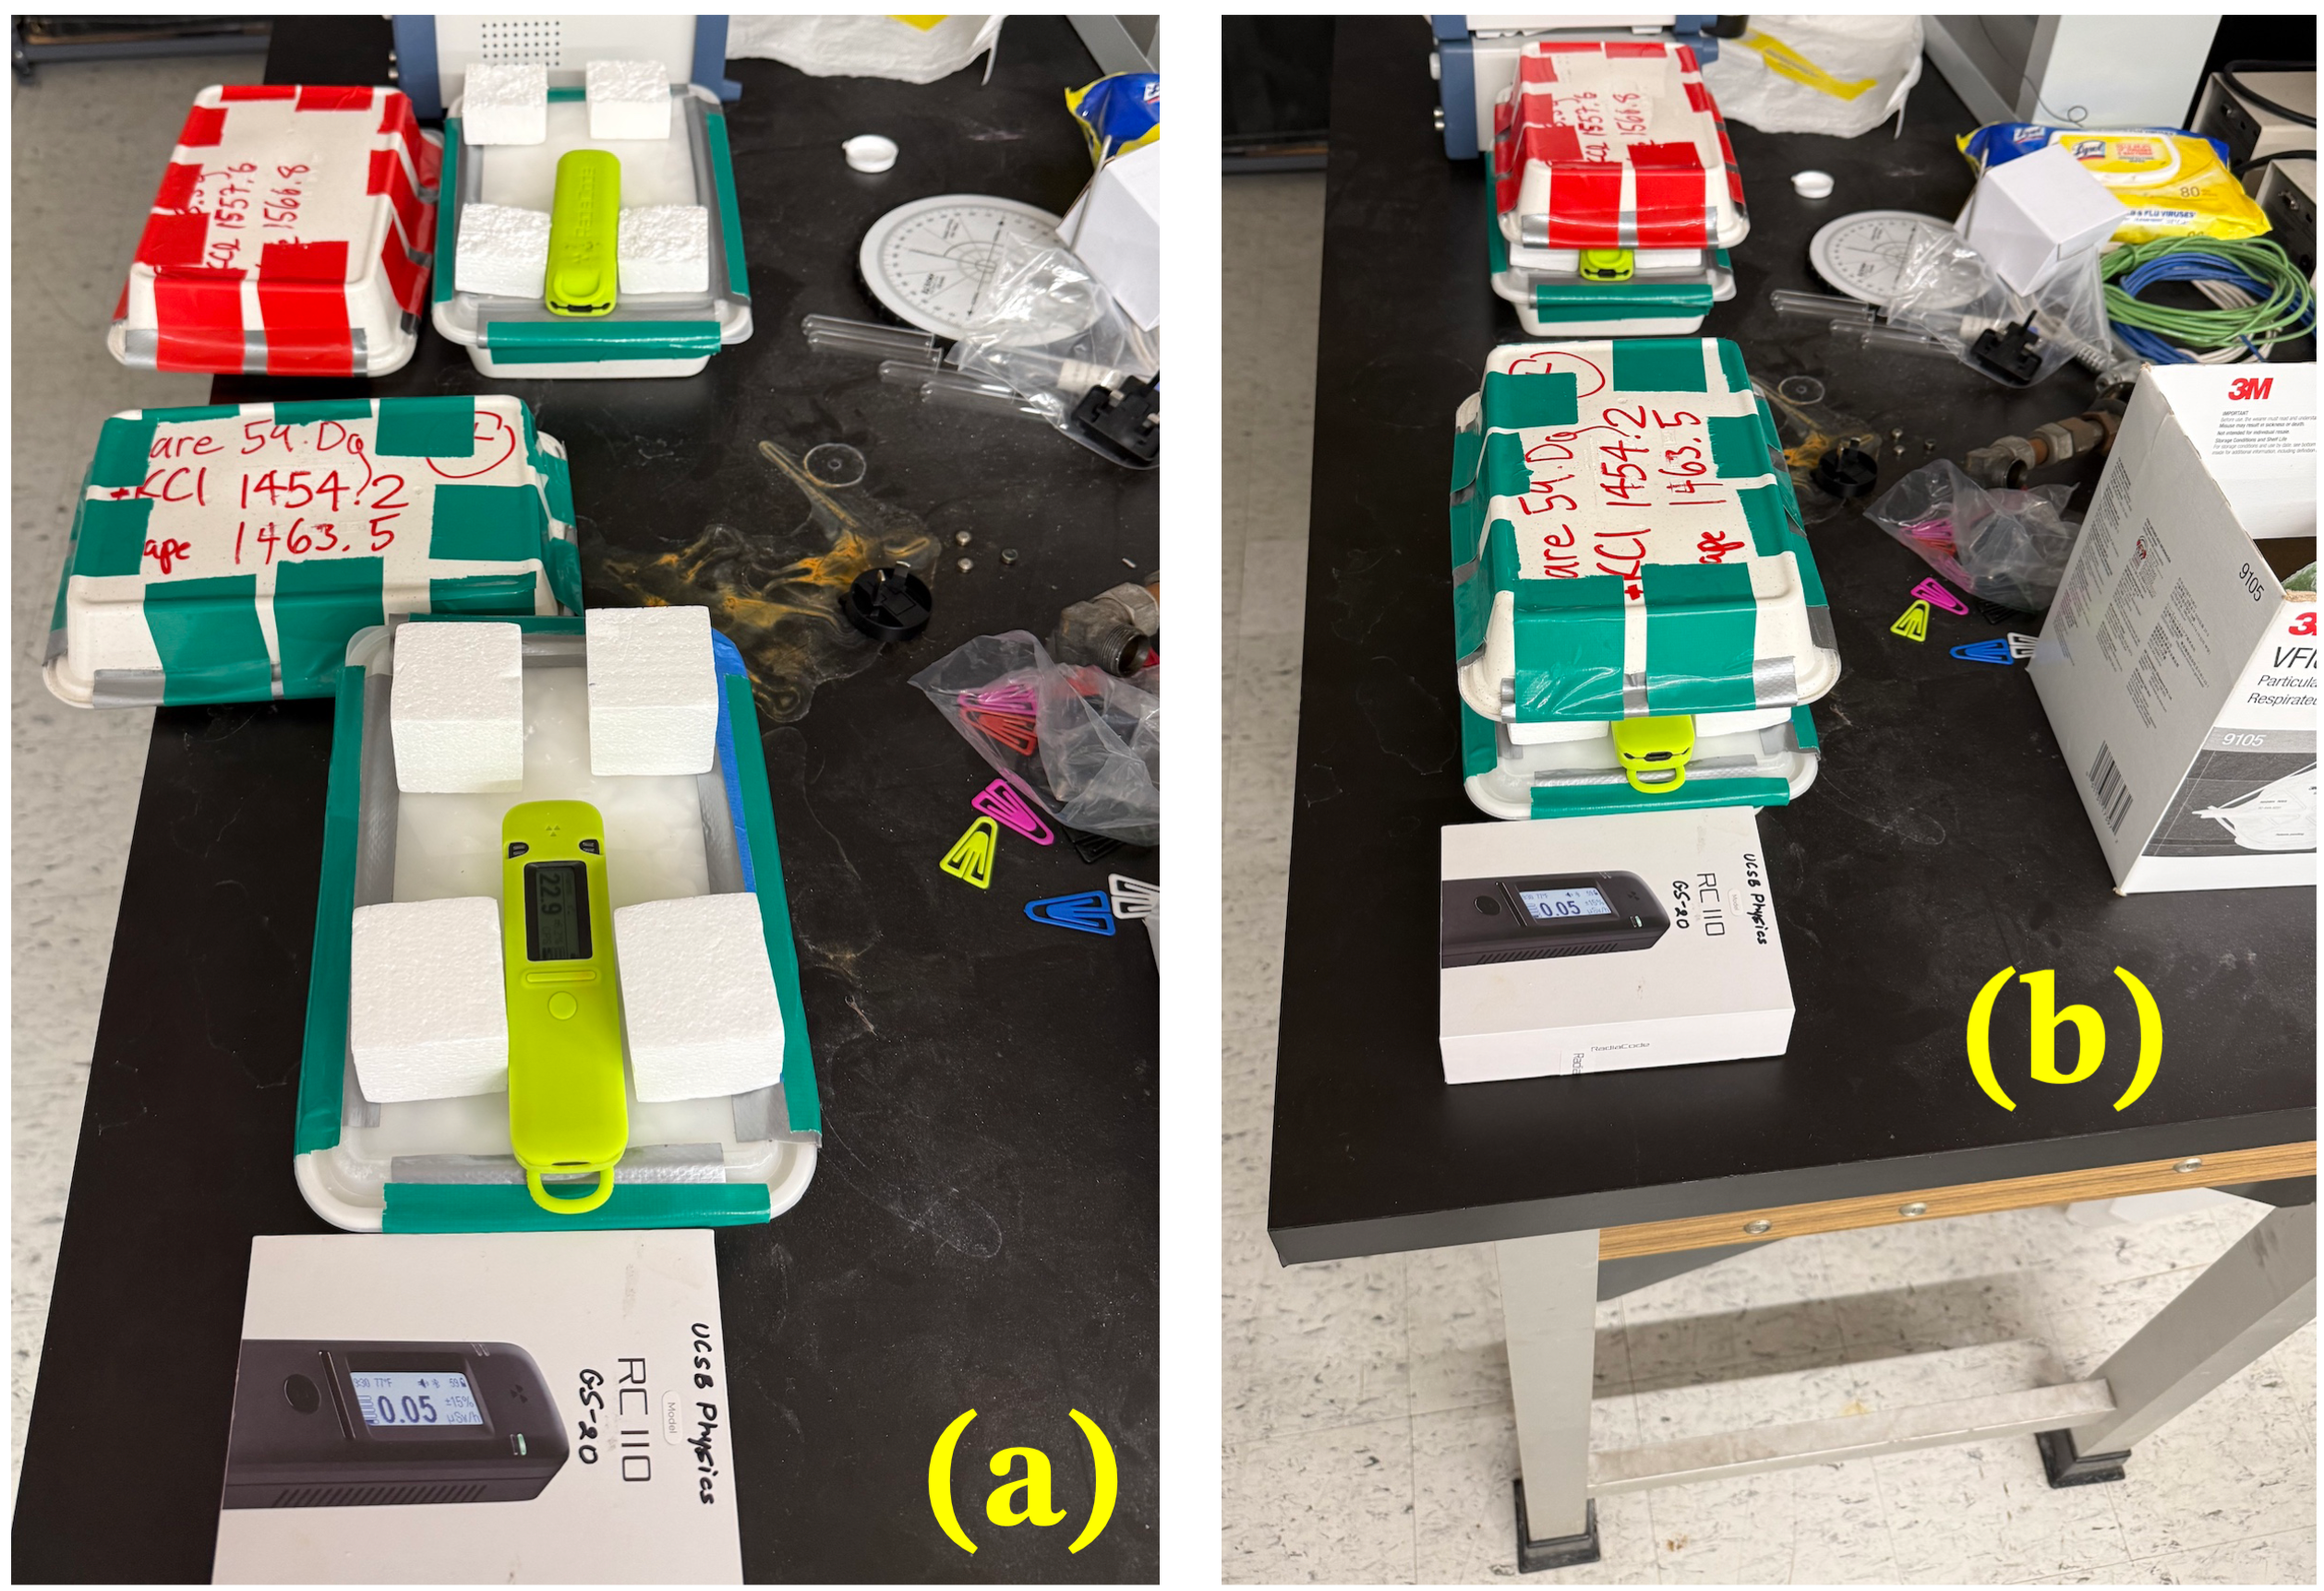
\includegraphics[width=0.75\textwidth]{KCl.png}
    \caption{(a)Radiacode position on bottom tray of KCl (b)second top tray in place}
    \label{fig:Kcl}
    \end{figure}
    \item (3 setups) \textbf{Potassium radioactivity}.  Measure radioactivity from common potassium by deploying the Radiacode between two food trays filled with KCl water-softening crystals, as shown in Fig.~\ref{fig:Kcl}.  A run for 20-60 minutes between the trays gives a good result, but, you must \emph{also} take a second \emph{background} run, of similar duration, because the room itself has gamma rays in it.  Take the background run in a location at least 3 meters from any other radioactivity.  You must subtract the ``room total rate" from that taken in the setups in Fig.~\ref{fig:Kcl} to get the pure KCl rate in counts per second, and then divide by the total cross section in CsI to deduce the flux, as you did in earlier labs. Also use the CsI information from \href{https://physics.nist.gov/PhysRefData/Xcom/html/xcom1.html}{XCOM} for the 1460~keV gamma's rate through photoelectric absorption, fit with Interspec as you did for Co-60, to deduce a flux of 1460~keV gammas.   Compare with the number of $\gamma$-rays per square-centimeter emitted from the food trays, where you need to do some Avogadro-number and lifetime/mean life math involving the \href{https://nds.iaea.org/relnsd/vcharthtml/VChartHTML.html}{IAEA table of nuclides}, to get the ``surface $\gamma$ ray flux".  By what (dimensionless) factor does the surface $\gamma$ ray flux exceed the measured flux from the Radiacode?  This factor is a result of geometry and self-absorption in the KCl.

    To help you with this lab, we have put a lot of information on environmental radioactivity in the second section of this lab guide.

    \begin{figure}[ht]
    \centering
    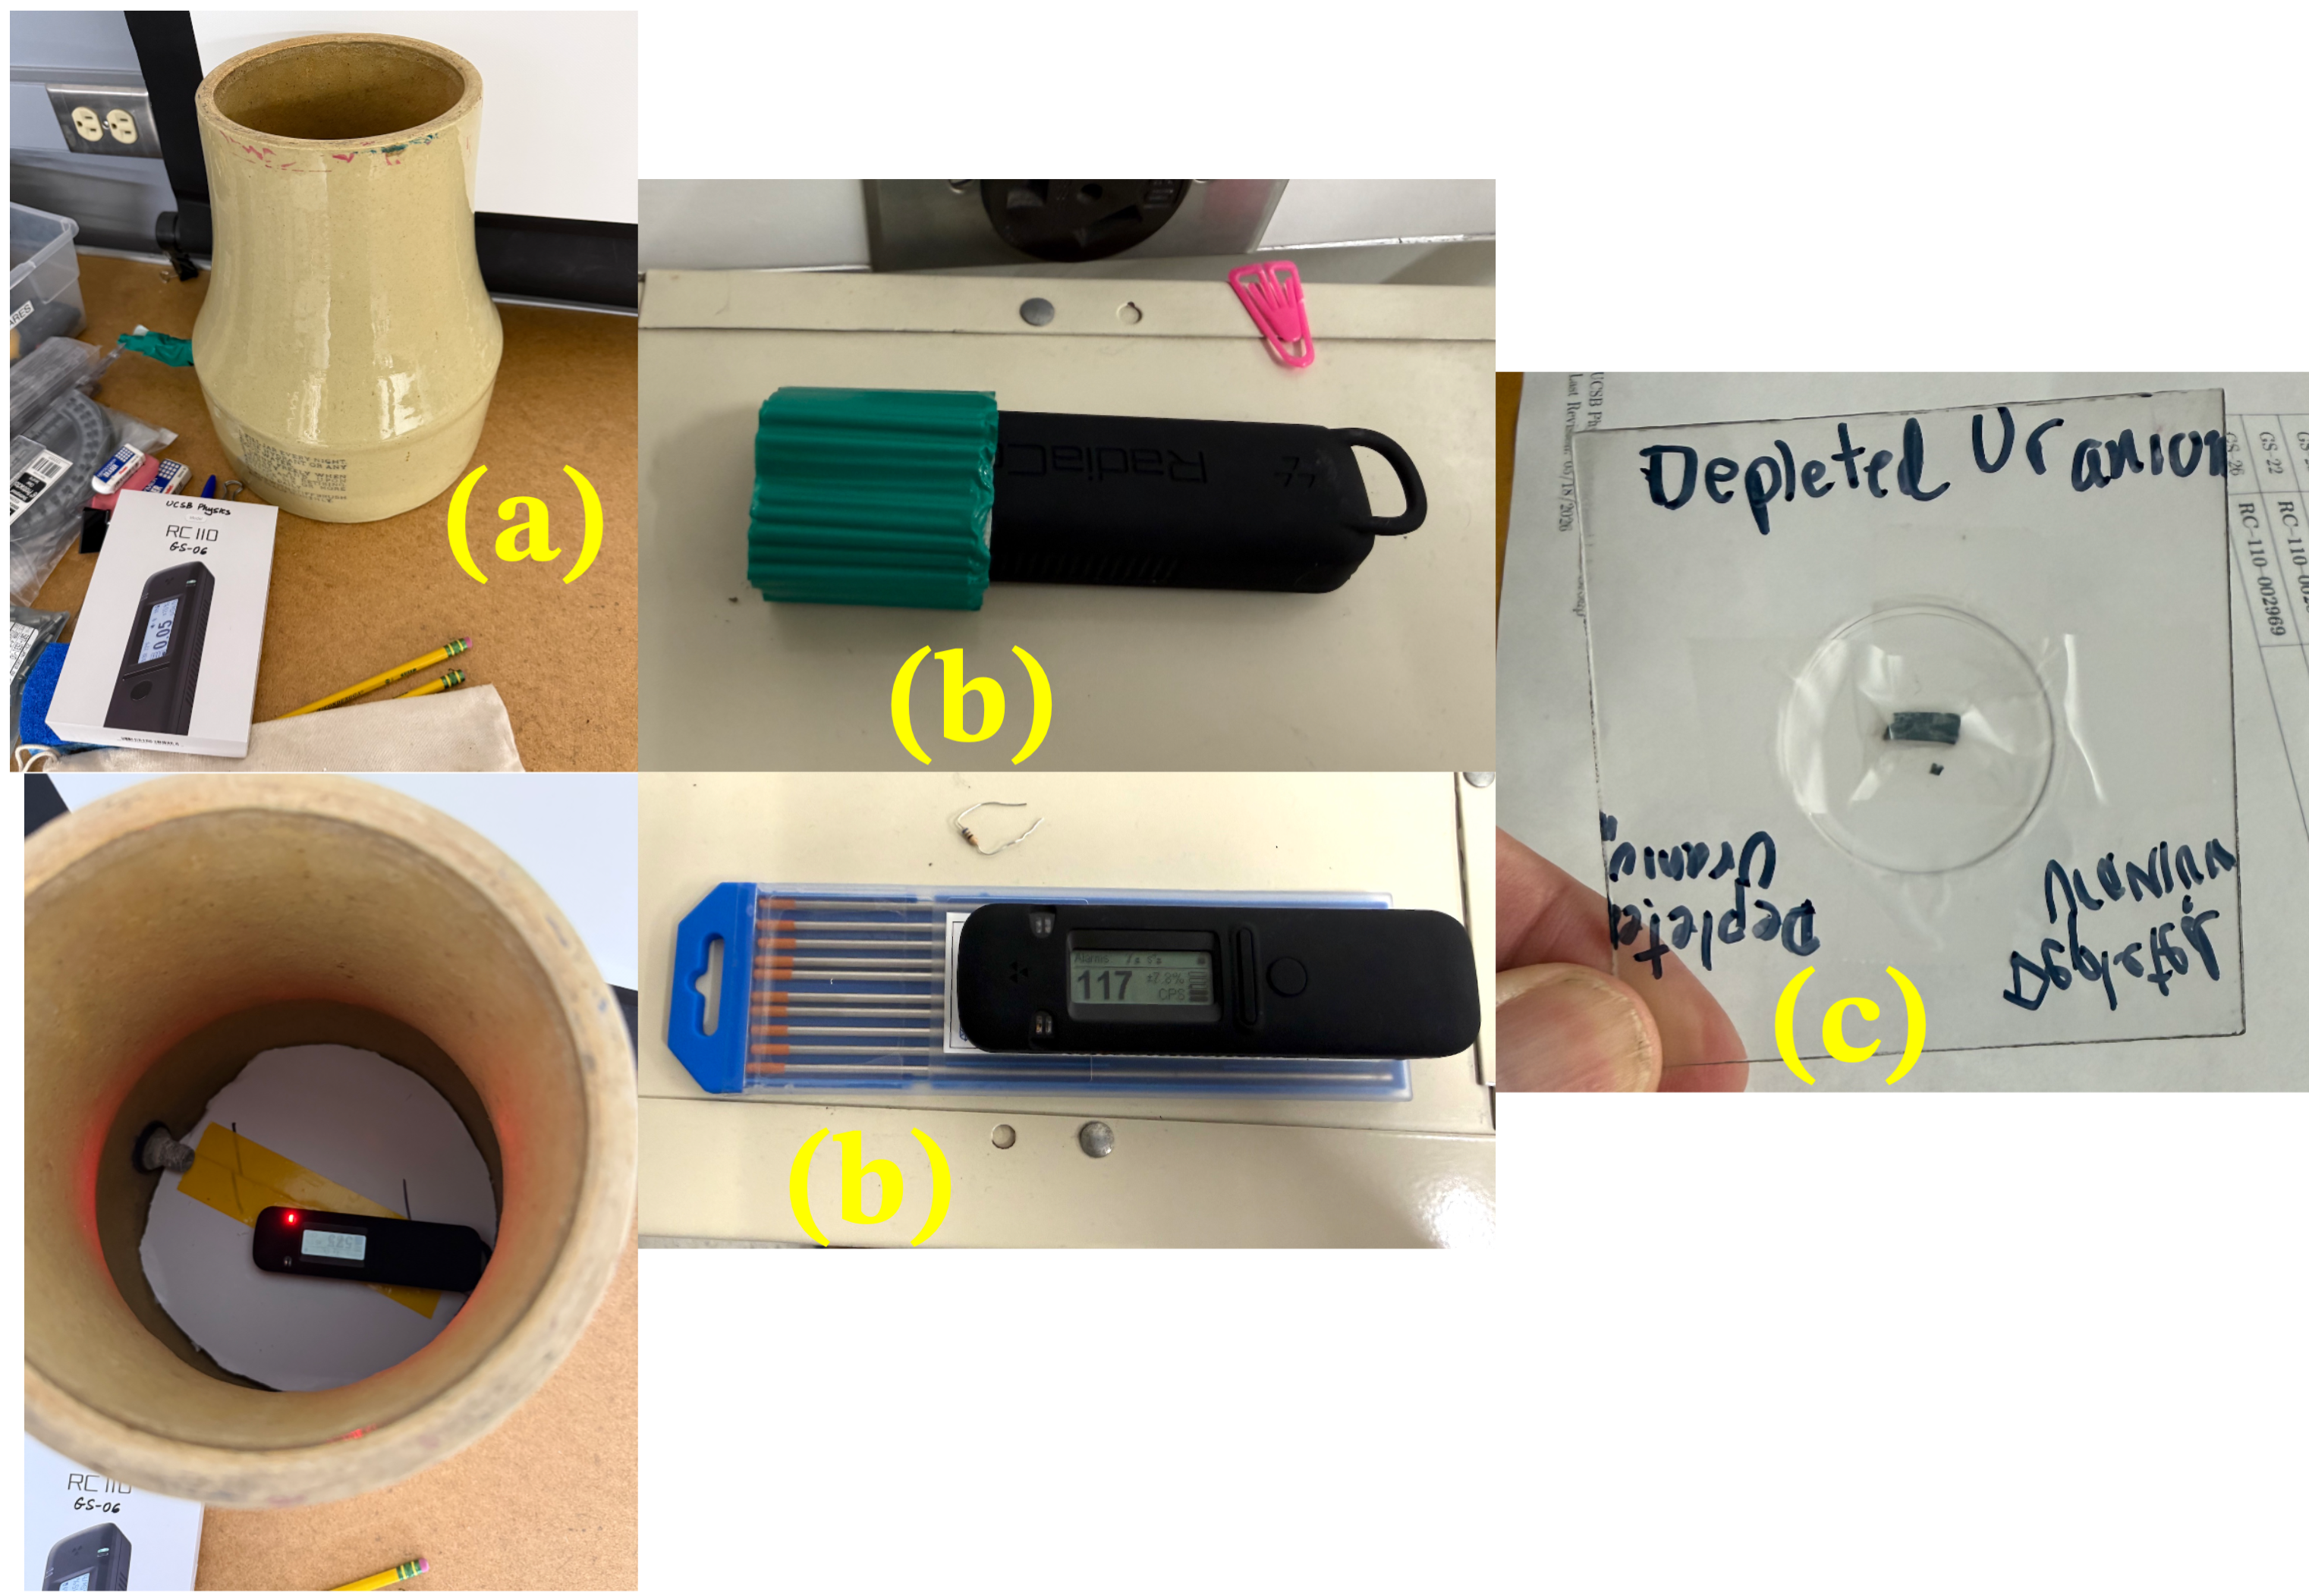
\includegraphics[width=0.75\textwidth]{HeaveElement.png}
    \caption{(a)Radium jar (several can deploy simultaneously) (b)thorium in welding rods (2 setups) (c)depleted uranium (only one source, measure in the ST-160 setup).}
    \label{fig:Heavy}
    \end{figure}
    \item (several setups) \textbf{Heavy element radioactivity.} Record the $\gamma$ spectra from 3 heavy mildly radioactive sources: radium, thorium, and depleted uranium, as shown in Fig.~\ref{fig:Heavy}.  Each spectrum should take about 20 minutes.  Upload into Interspec and identify as many peaks as you can. The minimum requirement is to make the figures like Fig.~\ref{fig:RadiumLow},  Fig.~\ref{fig:RadiumHigh}, and Fig.~\ref{fig:thorium} for each of the 3 sources, and fit the peaks shown there, to report the rates (in counts per second), and their spectrum. The plot from the single peak in depleted uranium is not shown in this guide; you must fit that peak and turn in that spectrum too.
    
    The decay chains of the heavy elements are complicated, but quite important for understanding radioactivity in our environment, as well as nuclear reactors and explosives.

    To help you with this lab, we have put a lot of information on environmental radioactivity in the second section of this lab guide.

    At the ``challenge" level, see if you can identify other $\gamma$ lines beyond those discussed in the second section, and understand the rates you measure by tracing back to a flux of decay products going through the CsI.  
    
    The ultimate interesting challenge: deduce the presence of positrons in the spectrum from thorium.  Details are in the section section, on thorium.

     \begin{figure}[ht]
    \centering
    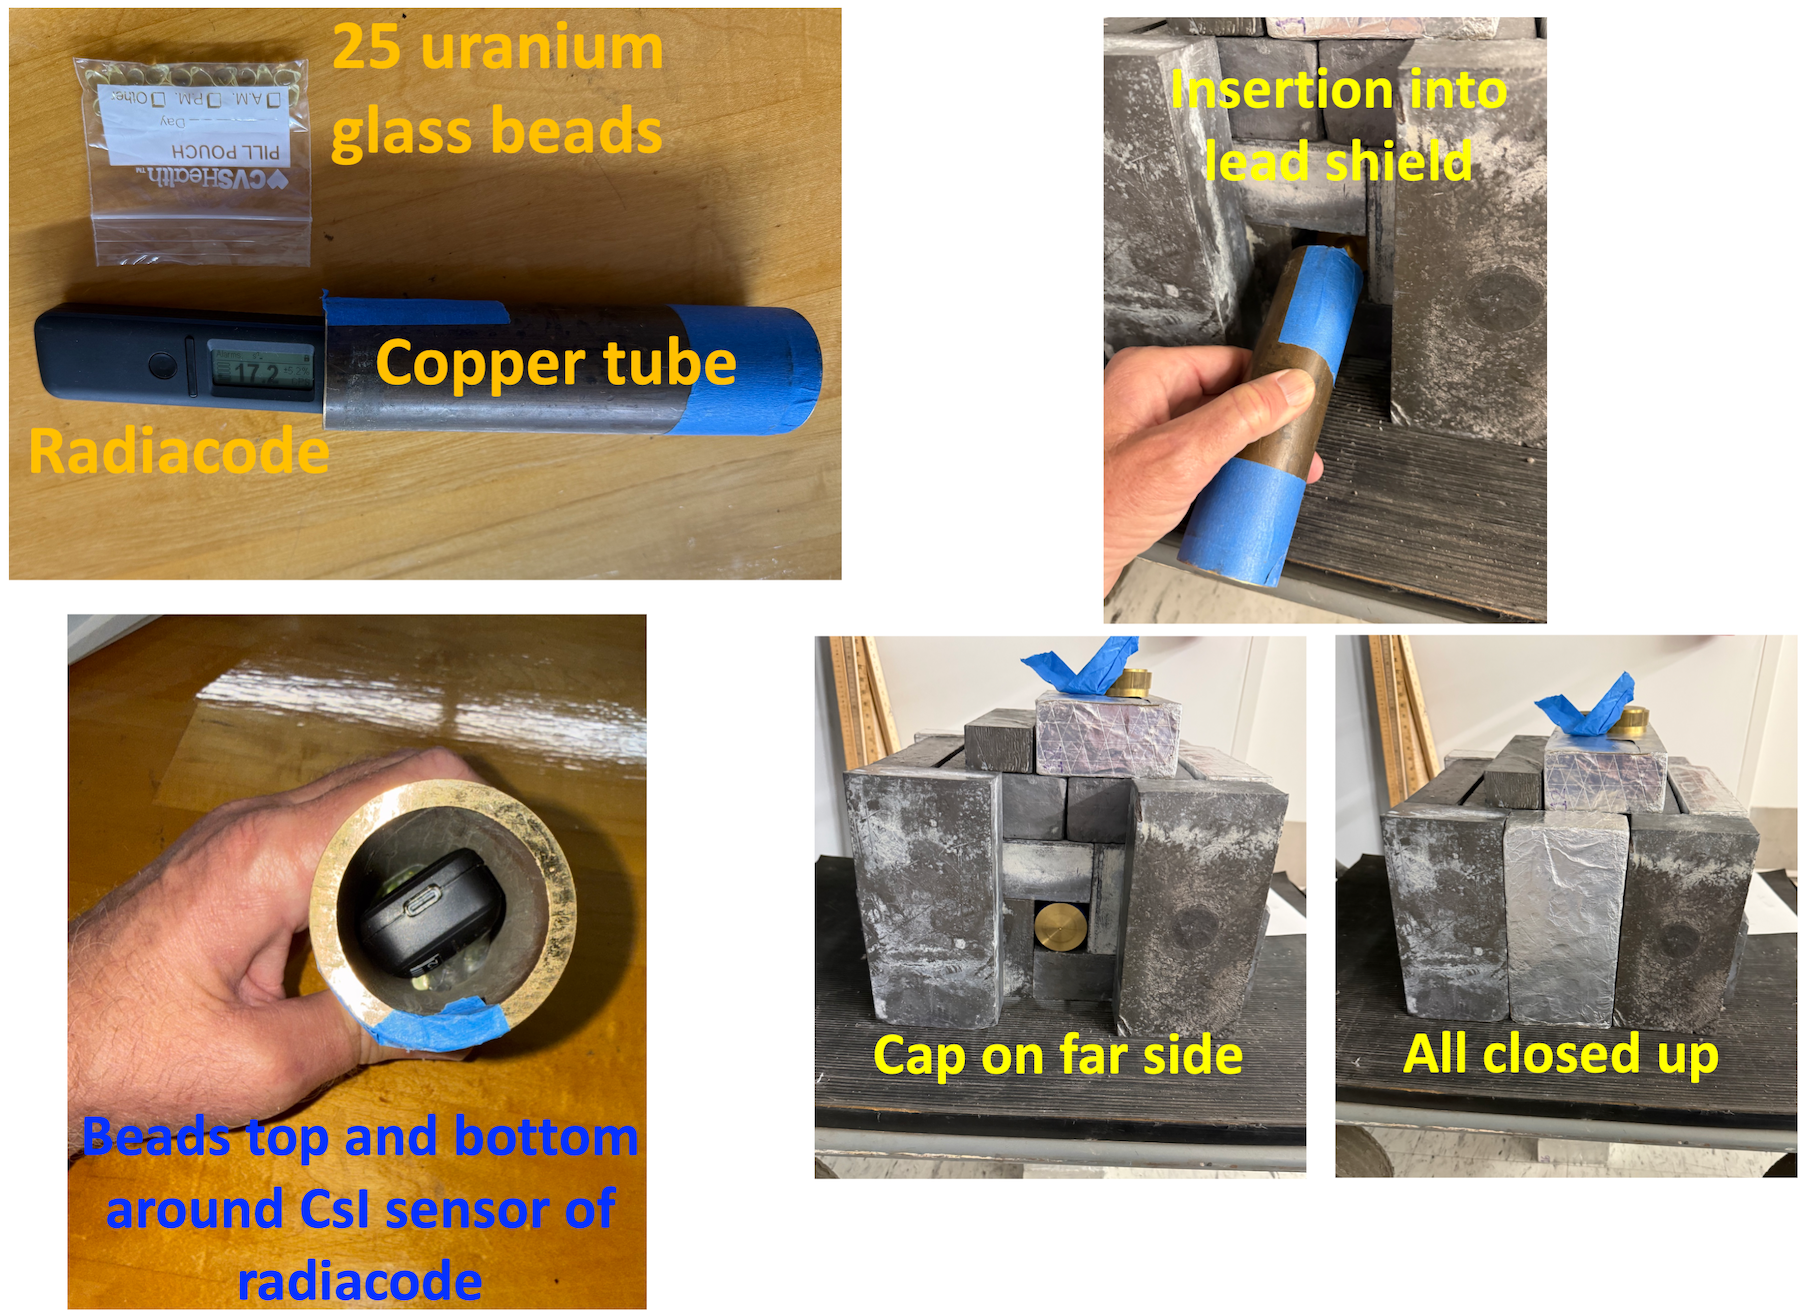
\includegraphics[width=0.75\textwidth]{LowBackground.png}
    \caption{The assembly for low background counting.  Note, you must do one run with no beads, and then a second with beads.  You'd like the runs to be about the same duration, and as long as you can fit into your lab period.}
    \label{fig:low}
    \end{figure}

\item (1 setup, could fit 2 students per lab period) \textbf{Low background counting}. The radiation environment of the room limits sensitivity of the Radiacode to small amounts of radioactivity. The small lead ``cave" at the front of class allows you to shield from much of the radioactivity of the lab room, and see signals more quickly and clearly than running out in the open in the room permits.  While the rate seen in your Radiacode just out in the room is 15-20 counts per second (cps), inside the lead cave, the rate is about 50 times lower, because the lead blocks most of the $\gamma$ rays that are emitted by materials in the room. Do 2 runs in the lead cave.  Only TAs can open/close the lead cave and its copper pipe.  The two runs are: nothing inside all other than the Radiacode, also known as ``background only".  You should see the lead fluorescence induced by external radioactivity, and some larger and smaller pulses in the spectrum.  Then put in the small packet Czech glass beads, purported to have depleted uranium in them.  A series of photos depicting the assembly is shown in Fig.~\ref{fig:low}.  Both runs should be a long in duration as possible, and each should have about then same duration.  Shoot for 45 minutes each. Can you identify the presence of depleted uranium?


    \begin{figure}[ht]
    \centering
    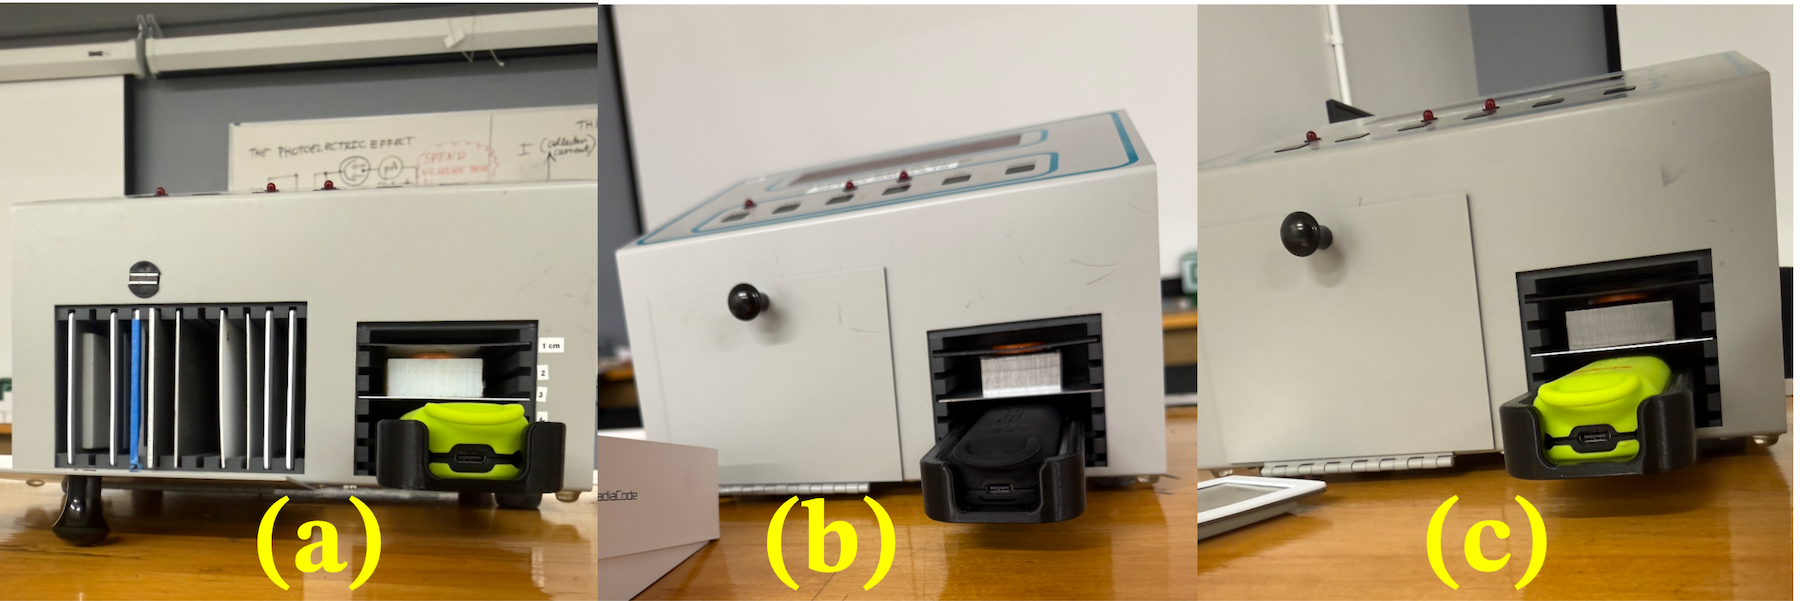
\includegraphics[width=0.75\textwidth]{Absorber.png}
    \caption{Absorbers: (a)nylon (b)aluminum (c)steel}
    \label{fig:absorber}
    \end{figure}

    \item (2 setups) \textbf{Cobalt-60 1332.5 gamma absorption}.
    As shown in Fig.~\ref{fig:absorber}, do the same absorption experiment you did for lead earlier, but for absorbers of nylon, aluminum, and steel.  You must measure the thickness of each absorber in gm/cm$^2$, by measuring their cross sectional area in square-centimeters, and weighing them to get the grams.  You must use XCOM to get the expected cross sections, and compare your data with expectation.  For nylon, you must find the chemical formula and use it in XCOM.
\end{enumerate}

\FloatBarrier
%\hbox{}
%\newpage
\section{Natural Radioactivity}

There are three principal categories of natural radioactivity:
\begin{enumerate}
    \item $\elem{K}{40}{19}{}{21}$.   Potassium is common on earth, where it is the eighth-most abundant element, and it is an essential nutrient in the human body.  The typical human body contains about 100~grams of potassium.   About $0.01177\,$\%, by moles, of natural potassium is $\elem{K}{40}{19}{}{21}$, which has a half-life of \qty{1.248E9}{y}.  About $10.55\,$\% of $\elem{K}{40}{19}{}{21}$ emit a $\gamma$ ray of energy \qty{1460.8}{keV}, which you can measure with the equipment in this lab
    \item Heavy (or actinide) decay chains.  There are four such chains, of which three occur naturally, and are labeled by their longest lived nuclides: $\elem{U}{238}{92}{}{146}$,  $\elem{Th}{232}{90}{}{142}$, and $\elem{U}{235}{92}{}{143}$.  These are the nuclides involved in nuclear reactors and explosives, and which are common in our environment.  You can measure the $\gamma$'s from these the $\elem{U}{238}{92}{}{146}$ and $\elem{Th}{232}{90}{}{142}$ in this lab.
    \item Cosmogenic nuclides, like $\elem{C}{14}{6}{}{8}$, which are continuously produced by naturally occuring nuclear reactions. $\elem{C}{14}{6}{}{8}$ is continuously produced by neutrons liberated by cosmic rays in the Earth's atmosphere. Due to $\elem{C}{14}{6}{}{8}$'s short half-life of 5,700~y, it has been used to date many relics of human civilizations.  We do nothing with $\elem{C}{14}{6}{}{8}$ in this lab. 
\end{enumerate}


\subsection{Potassium-40}

 \begin{figure}[ht]
    \centering
    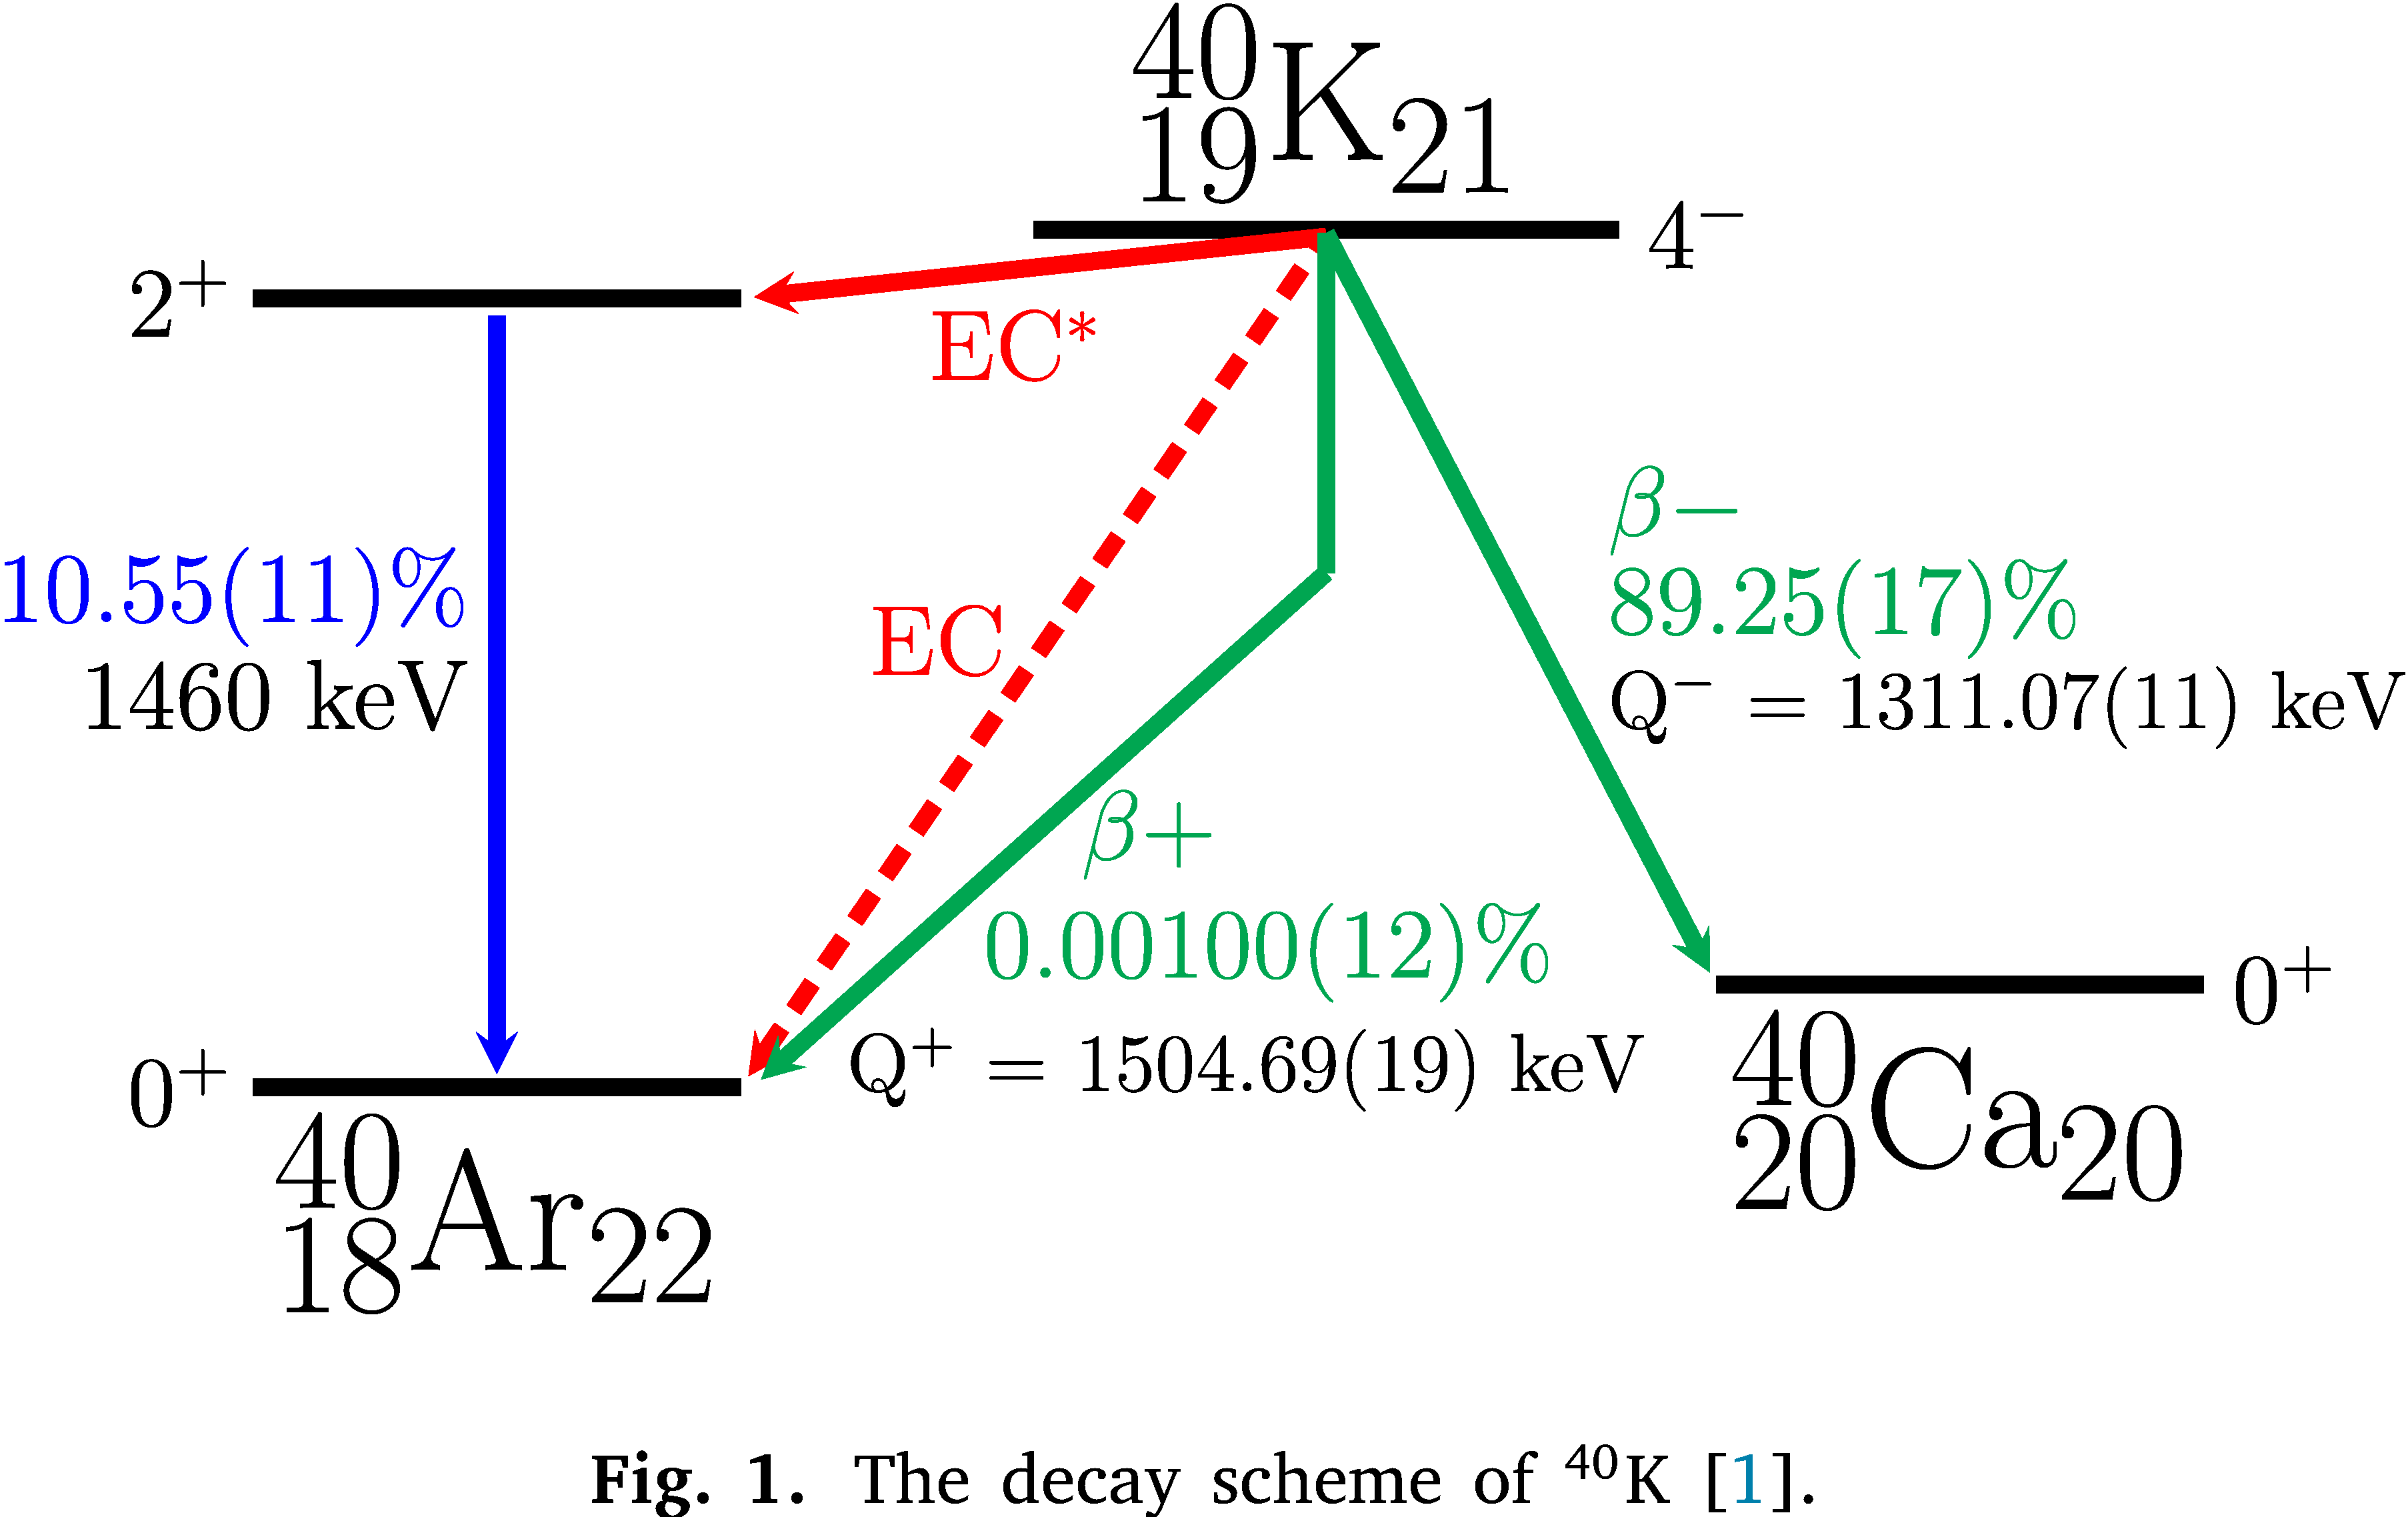
\includegraphics[width=0.75\textwidth]{40KDecayScheme.png}
    \caption{The decays of $\elem{K}{40}{19}{}{21}$.  About $89\,$\% of the time, $\elem{K}{40}{19}{}{21}$ undergoes $\beta$ decay to $\elem{Ca}{40}{20}{}{20}$.  In the other $11\,$\% of decays,  $\elem{K}{40}{19}{}{21}$ undergoes \emph{electron capture}, or, $\beta^+$ decay, to give $\elem{Ar}{40}{18}{}{22}$, and in that case, usually emits a $\gamma$ ray.  Most argon in the Earth's atmosphere originates from the decay of $\elem{K}{40}{19}{}{21}$.}
    \label{fig:potas}.
    \end{figure}

A diagram showing the three mechanisms by which $\elem{K}{40}{19}{}{21}$ can decay is given in Fig.~\ref{fig:potas}.  $\elem{K}{40}{19}{}{21}$ can decay in three distinct manners, and again, quantum mechanics renders impossible, as far as we know, any ability to predict which decay will be selected by an particular potassium atom.  The three manners are:

\begin{enumerate}
\item Standard $\beta$ decay, in about 89~\% of decays: $\elem{K}{40}{19}{}{21}\!\to\!\elem{Ca}{40}{20}{+}{20}+e^-+\overline{\nu}_e$
\item Positron or $\beta^+$ decay, very rarely, in about 0.001~\% of decays: $\elem{K}{40}{19}{}{21}\!\to\!\elem{Ar}{40}{18}{-}{22}+e^++\nu_e$.  The positron, $e^+$, is the antimatter partner of the electron, with the same mass, but opposite charge.  If a positron and electron meet, they annihilate, and emit a burst of $\gamma$ rays.  The $\nu_e$ is the antimatter partner of the electron antineutrino.  In fact, in the thorium chain, you can see evidence of positron annihiliation via escape features.
\item \emph{Electron capture}: $\elem{K}{40}{19}{}{21}+e^-\!\to\!\elem{Ar}{40}{18}{}{22}+\nu_e$.  Electron capture happens when the $\elem{K}{40}{19}{}{21}$ nucleus absorbs an atomic electron, usually from the electron orbit that is most tightly bound to the nucleus. About $11\,$\% of $\elem{K}{40}{19}{}{21}$ nuclides decay by electron capture.  Electron capture is related to $\beta^+$ decay by a concept of \emph{crossing}: crossing describes taking a particle from the final state (in this case, the positron) and crossing it to the initial state, and flipping its matter-antimatter property.   Angular momentum considerations greatly favor the $\elem{K}{40}{19}{}{21}$ state that is excited, and when this state decays, a $\gamma$ ray of energy 1460.8~keV is emitted.
\end{enumerate}

\subsection{Heavy (Actinide) decay chains}

The two main actinide decay are shown in Fig.~\ref{fig:uchain} for $\elem{U}{238}{92}{}{146}$, and Fig.~\ref{fig:thchain} for 
$\elem{Th}{232}{90}{}{142}$.

The actinide decay chains are complicated, and take some time to absorb, but, they are quite important in a wide variety of scientific fields, from geology to the search for dark matter.

\begin{sidewaysfigure}
    \centering
    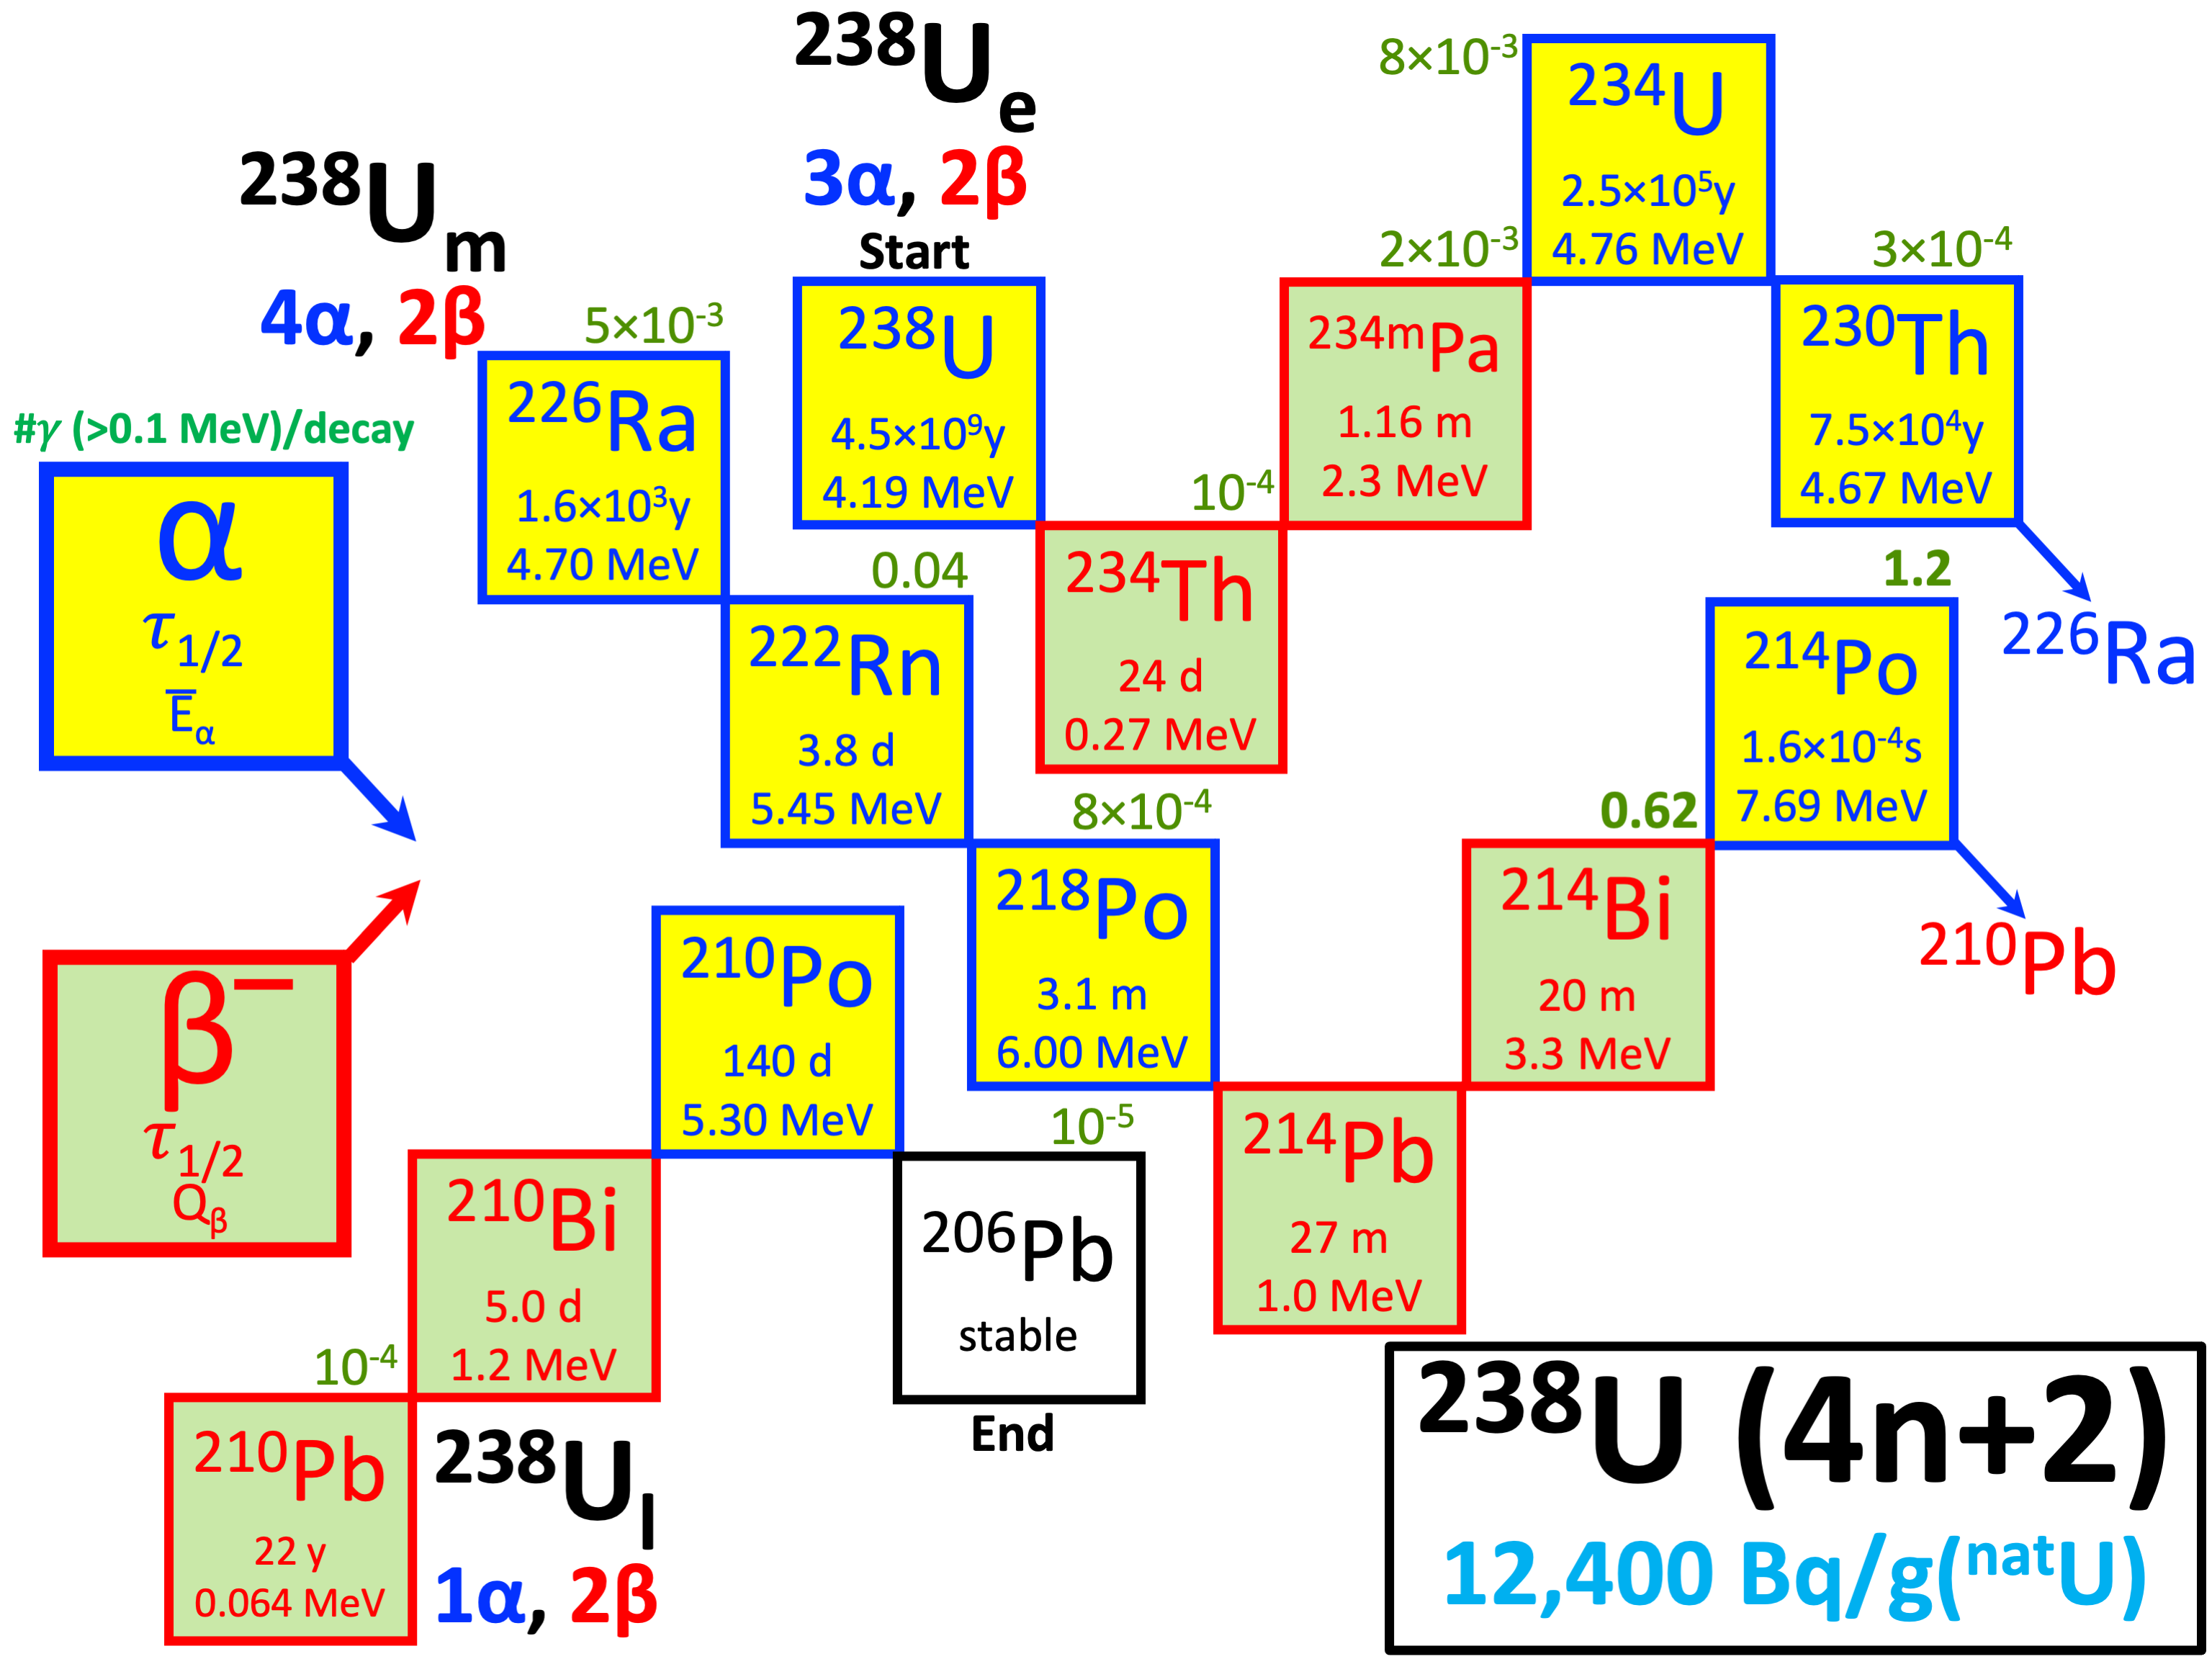
\includegraphics[width=0.95\textheight]{U238Chain.png}
    \caption{The $\elem{U}{238}{92}{}{146}$ decay chain.  The green numbers above each box show how many $\gamma$ rays are emitted per decay.  The way to read the chart is: the $\beta$ decay of $\elem{Bi}{214}{83}{}{131}$ goes to an excited state of $\elem{Po}{214}{84}{}{131}$, which on average emit 1.2 $\gamma$ rays per $\beta$ decay.  More than one $\gamma$ per $\beta$ decay can be emitted because there is often a cascade of multiple $\gamma$'s as the excited $\elem{Po}{214}{84}{}{131}$ decays.}
    \label{fig:uchain}
\end{sidewaysfigure}

\subsubsection{The uranium chain}

The $\elem{U}{238}{92}{}{146}$ chain is shown in Fig~\ref{fig:uchain}.  It starts in the upper middle, in the blue and yellow box with $\elem{U}{238}{}{}{}$. 

A blue and yellow box indicates that the nuclide in its label undergoes $\alpha$ decay.  $\alpha$ decay is one of the first known cases of quantum-mechanical tunneling: it appears that the $\alpha$-particle, on its way out of the nucleus, seems to briefly violate energy conservation.  It is the quantum mechanical wave nature of the $\alpha$ particle that permits the apparent brief violation of energy conservation.

An $\alpha$-particle is the nucleus of a helium atom, $\elem{He}{4}{2}{2+}{2}$.  When $\elem{U}{238}{92}{}{146}$ decays, the reaction is:
\begin{equation*}
\elem{U}{238}{92}{}{146}\!\to\!\elem{Th}{234}{90}{}{144}+\elem{He}{4}{2}{2+}{2}+2e^-
\end{equation*}
The kinetic energy of the emitted $\elem{He}{4}{2}{2+}{2}$, from Fig.~\ref{fig:uchain}, is 4.19~MeV.  The $\elem{Th}{234}{90}{}{144}$ nucleus is so heavy that it carries away little energy, although by conservation of momentum, it carries away nearly the same amount of momentum as the $\alpha$ particle.  Kinetic energy is $\propto p^2/(2m)$, where $m$ is mass, ans so the huge mass in $\elem{Th}{234}{90}{}{144}$ suppresses its kinetic energy.  The two electrons do very little.

The geometric layout used in Fig.~\ref{fig:uchain} is simply for convenience: it is not a nuclide chart.  In $\alpha$ decay, the final nucleus has 4~units lower atomic mass number, 2~units lower atomic number, and 2 fewer neutrons.  The green and red boxes in Fig.~\ref{fig:uchain} indicate $\beta$ decay, where the final nucleus has the same atomic mass number of the initial nucleus, the atomic number increases by one, and the neutron number decreases by one.

\begin{figure}
    \centering
    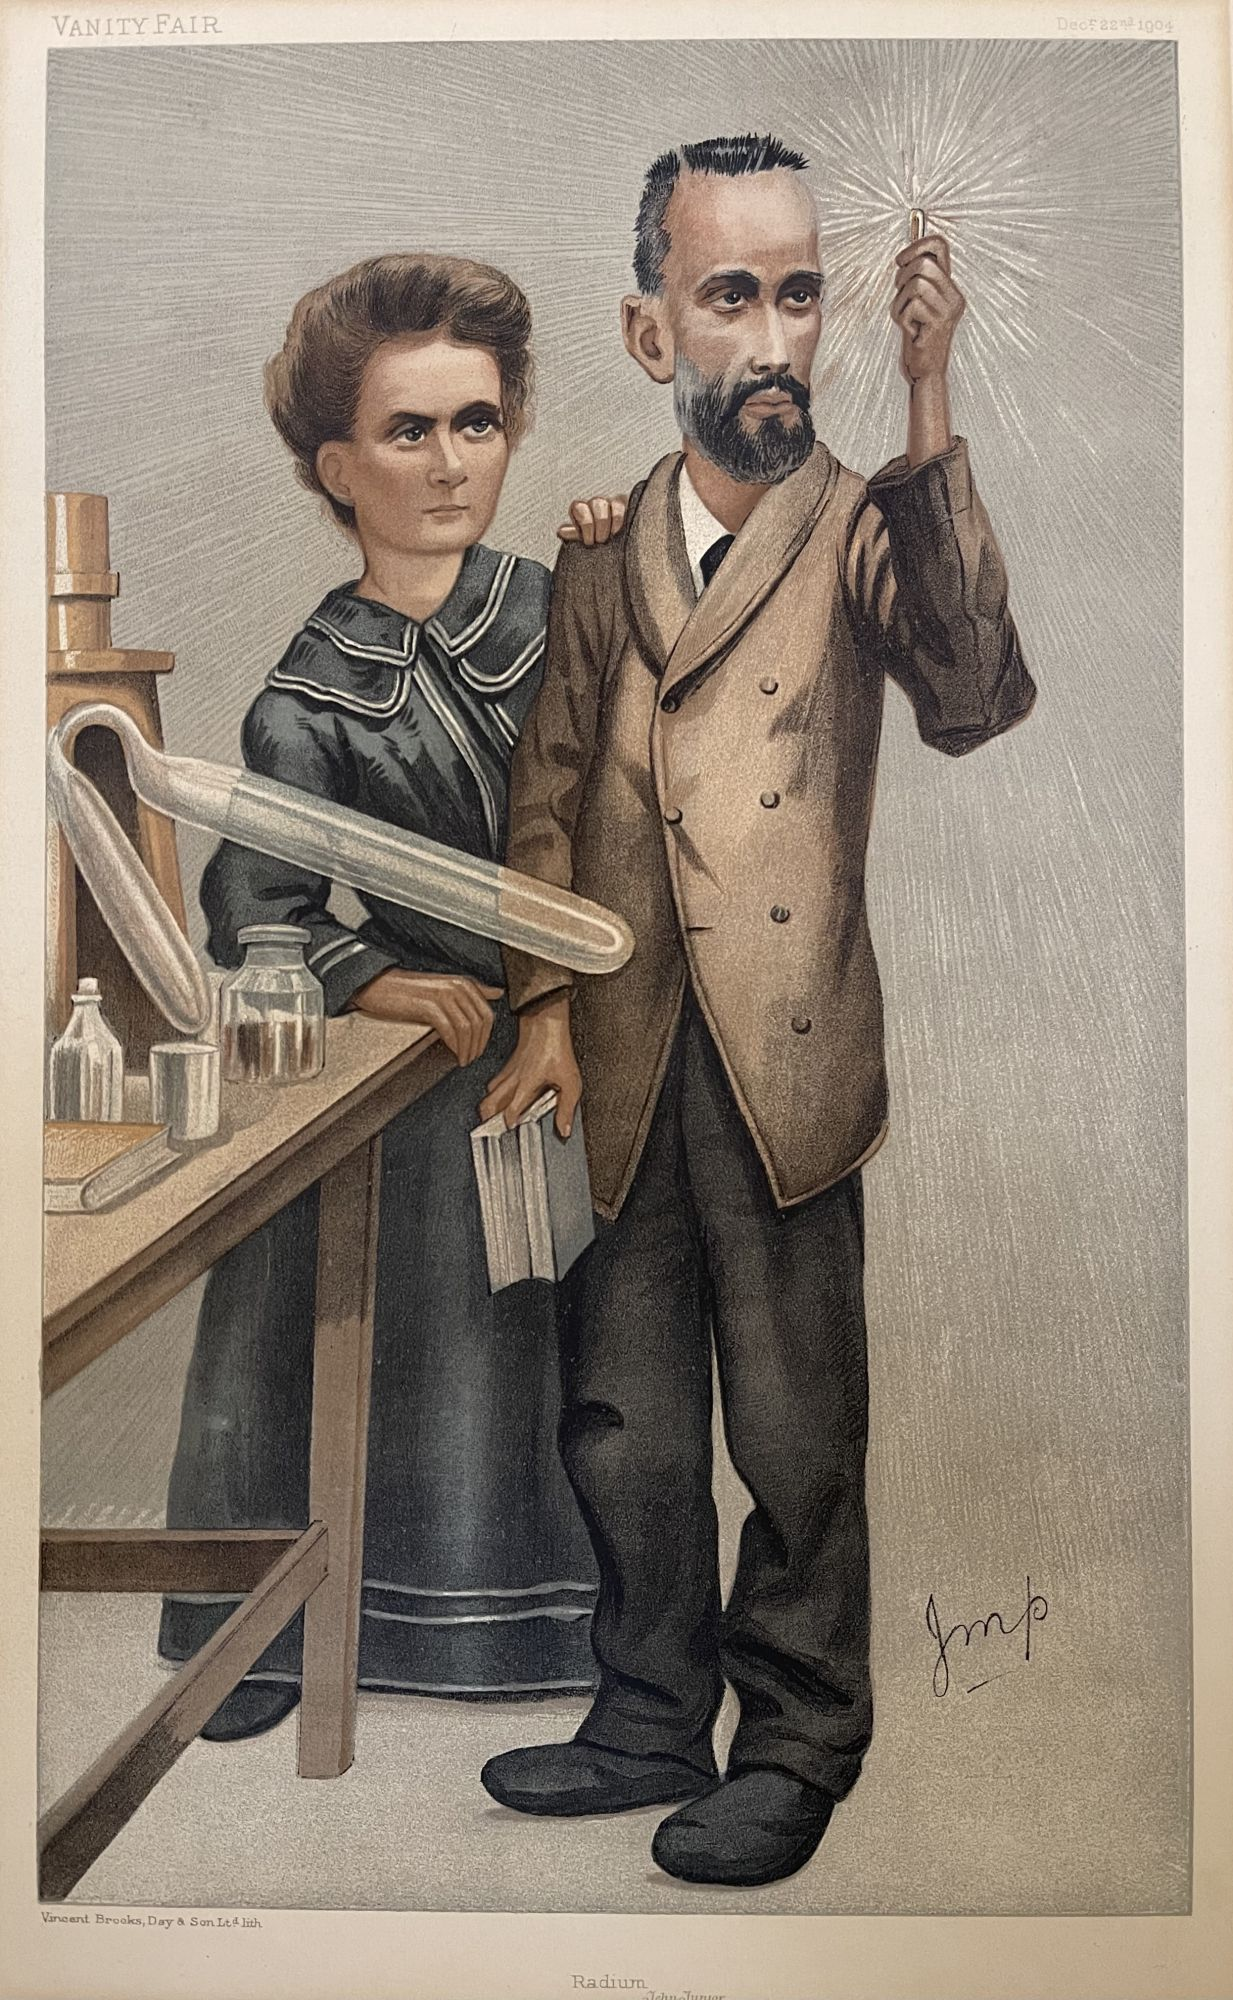
\includegraphics[width=0.76\textwidth]{RadiumCuries.jpg}
    \caption{Marie and Pierre Curie, with Pierre holding a luminous vial of radium, from a December, 1904 Vanity Fair magazine.}
    \label{fig:radium}
\end{figure}

Fig~\ref{fig:uchain} describes a sequence of 14 decays that starts at $\elem{U}{238}{92}{}{146}$, and then proceeds through 8~$\alpha$ decays and 6~$\beta$ decays to the stable nuclide $\elem{Pb}{206}{82}{}{124}$.   Some of the nuclides in the sequence have been very important:
\begin{itemize}
    \item $\elem{U}{238}{92}{}{146}$, which Becquerel discovered caused radioactivity, in 1896. His signal actually resulted from the high-energy $\beta$ decays in the chain in Fig.~\ref{fig:uchain}. Before it was known to be radioactive, uranium was used in ceramics and glass. In glass, it provides a greenish/yellowish tint. $\elem{U}{238}{92}{}{146}$ is used in nuclear reactors, where after capture of a neutron, eventually gives plutonium, $\elem{Pu}{239}{94}{}{145}$.  The first large-scale reactors were developed during the Manhattan Project in the 1940's. 
    
   $\elem{U}{238}{92}{}{146}$ starts the ``early" portion of the uranium chain, $\elem{U}{238}{}{}{\text{e}}$, in which there are 3$\alpha$ and 2$\beta$ decays. Most processed uranium you can purchase in the US has only has early part of the chain present, because nuclides with atomic mass number less than or equal to 235 have been removed, and is usually known as ``depleted uranium".  The lighter nuclides have been removed by US government processing to separate out and hold back $\elem{U}{235}{92}{}{143}$, which can be used to make a nuclear fission explosive.  
   
   There is only one clear $\gamma$ ray in the $\elem{U}{238}{}{}{\text{e}}$ portion of the chain, and it is from a very interesting process, the $\beta$-decay of an unusual excited nuclide known as a ``metastable isomer" $\elem{Pa}{234\text{m}}{91}{}{143}$, to an excited state of $\elem{U}{234}{92}{}{142}$, which then decays through emission of a $\gamma$ ray of energy 1001.0~keV.  That is the $\gamma$ ray to look for when you use the Radiacode to look at the depleted uranium source.  The \href{https://www-nds.iaea.org/relnsd/vcharthtml/VChartHTML.html#&showtype=2&lastnuc=208Tl&tabid=NR}{IAEA Table of Nuclides} lists this gamma under its entry for the parent, $\elem{Pa}{234\text{m}}{91}{}{143}$.

    \item $\elem{Ra}{226}{88}{}{138}$, discovered by the Curies (see Fig.~\ref{fig:radium}).  Radium was used for many years to make glow-in-the-dark watch dials and other instrument dials.  Since the half-life of $\elem{Ra}{226}{88}{}{138}$ is 1603~years, products made with radium after 1900 are still radioactive, although the compounds used to create the glow have often become less effective.  Vintage radium dial products can be purchased in eBay. 
    
    The radium jar used in our experiment was made in about 1920, and its radium is immobile, backed into the ceramic at the bottom of the jar.  The bottom of the jar is covered by a plastic barrier.  The jar dates from the time in history when radium was thought to be a miracle substance, described in \href{https://youtu.be/83rd7eqxIHQ?si=QGlCiXy1jSI9tWp-}{this Youtube video}.  The jar we have is safe.
    
    $\elem{Ra}{226}{88}{}{138}$ starts the ``middle" portion of the chain, $\elem{U}{238}{}{}{\text{m}}$.  Most of the $\gamma$ rays you will detect upon deploying in the radium jar are from this portion of the decay sequence.
    One comes from $\elem{Ra}{226}{88}{}{138}$ $\alpha$ decay to an excited state of $\elem{Rn}{222}{86}{}{136}$, which then decays through emission of a 186.2~keV $\gamma$ ray.  Because the radium jar has a lot of radium in it (although not an unsafe amount), this line is prominent in the Radiacode.  Additionally, there are many $\gamma$ rays from the decays of excited states of $\elem{Bi}{214}{83}{}{131}$ and $\elem{Po}{214}{82}{}{131}$, and can be found on the \href{https://www-nds.iaea.org/relnsd/vcharthtml/VChartHTML.html#&showtype=2&lastnuc=208Tl&tabid=NR}{IAEA Table of Nuclides} under the respective parents, $\elem{Pb}{214}{82}{}{132}$ and $\elem{Bi}{214}{83}{}{131}$.
    
    \item $\elem{Rn}{222}{86}{}{136}$ is the main isotope of radon which can make basements in certain places in the world dangerously radioactive. Since radon is a noble gas, it escapes from solids.  Both radon and radium are substantial contributors to cancer caused by tobacco use.
    
    \item $\elem{Pb}{210}{82}{}{128}$, the beginning of the late chain, $\elem{U}{238}{}{}{\text{l}}$.  The implantation of $\elem{Pb}{210}{82}{}{128}$ surfaces can be used to determine lifetime exposure of those surfaces to radon gas.
    
     \item $\elem{Bi}{210}{83}{}{127}$, the nuclide used by physicists Ellis and Wooster to perform the experiment which resulted in the introduction of the neutrino particle.
     
     \item $\elem{Po}{210}{84}{}{126}$, used originally to initiate nuclear fission-based explosions, and as a \href{https://en.wikipedia.org/wiki/Alexander_Litvinenko}{hard-to-detect poison}.
      \item $\elem{Pb}{206}{82}{}{124}$, used to date rocks on Earth.
\end{itemize}

\begin{sidewaysfigure}
    \centering
    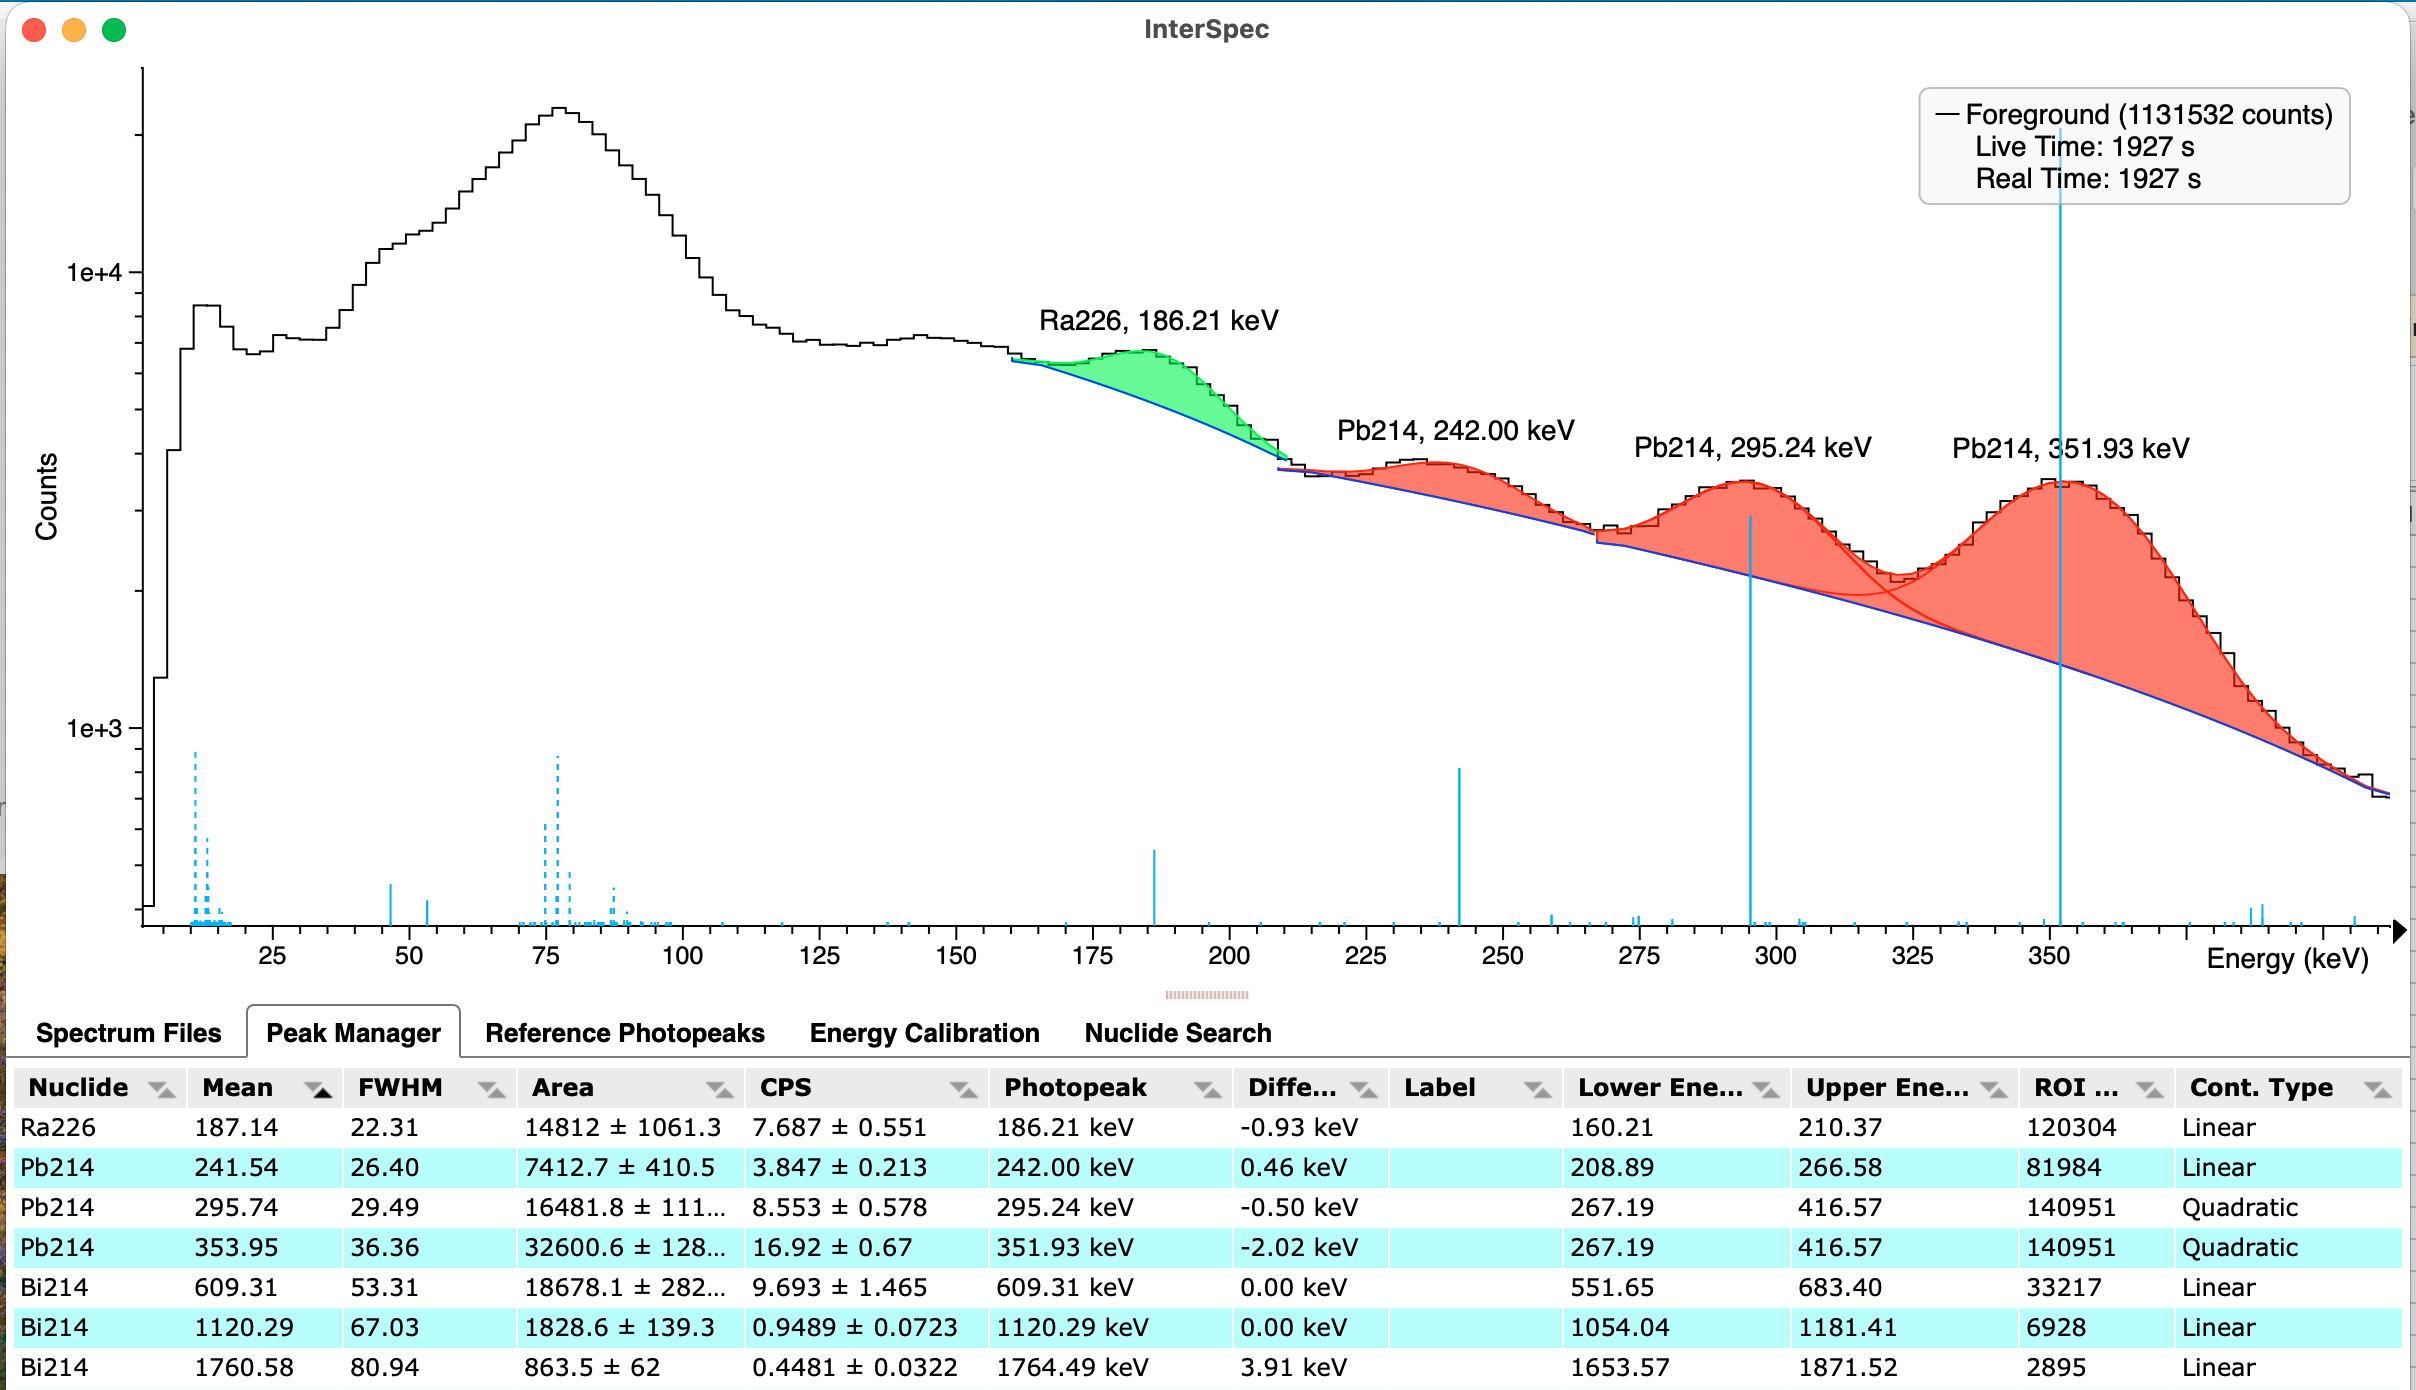
\includegraphics[width=0.95\textheight]{RadiumLow.png}
    \caption{Typical low energy portion of the spectrum from measurement of the Radiacode in the radium jar. At a minimum you should report your measurements of the 7 $\gamma$ rays shown at the bottom of the figure, and described in Tab.~\ref{tab:radiumgam}.}
    \label{fig:RadiumLow}
\end{sidewaysfigure}

\begin{sidewaysfigure}
    \centering
    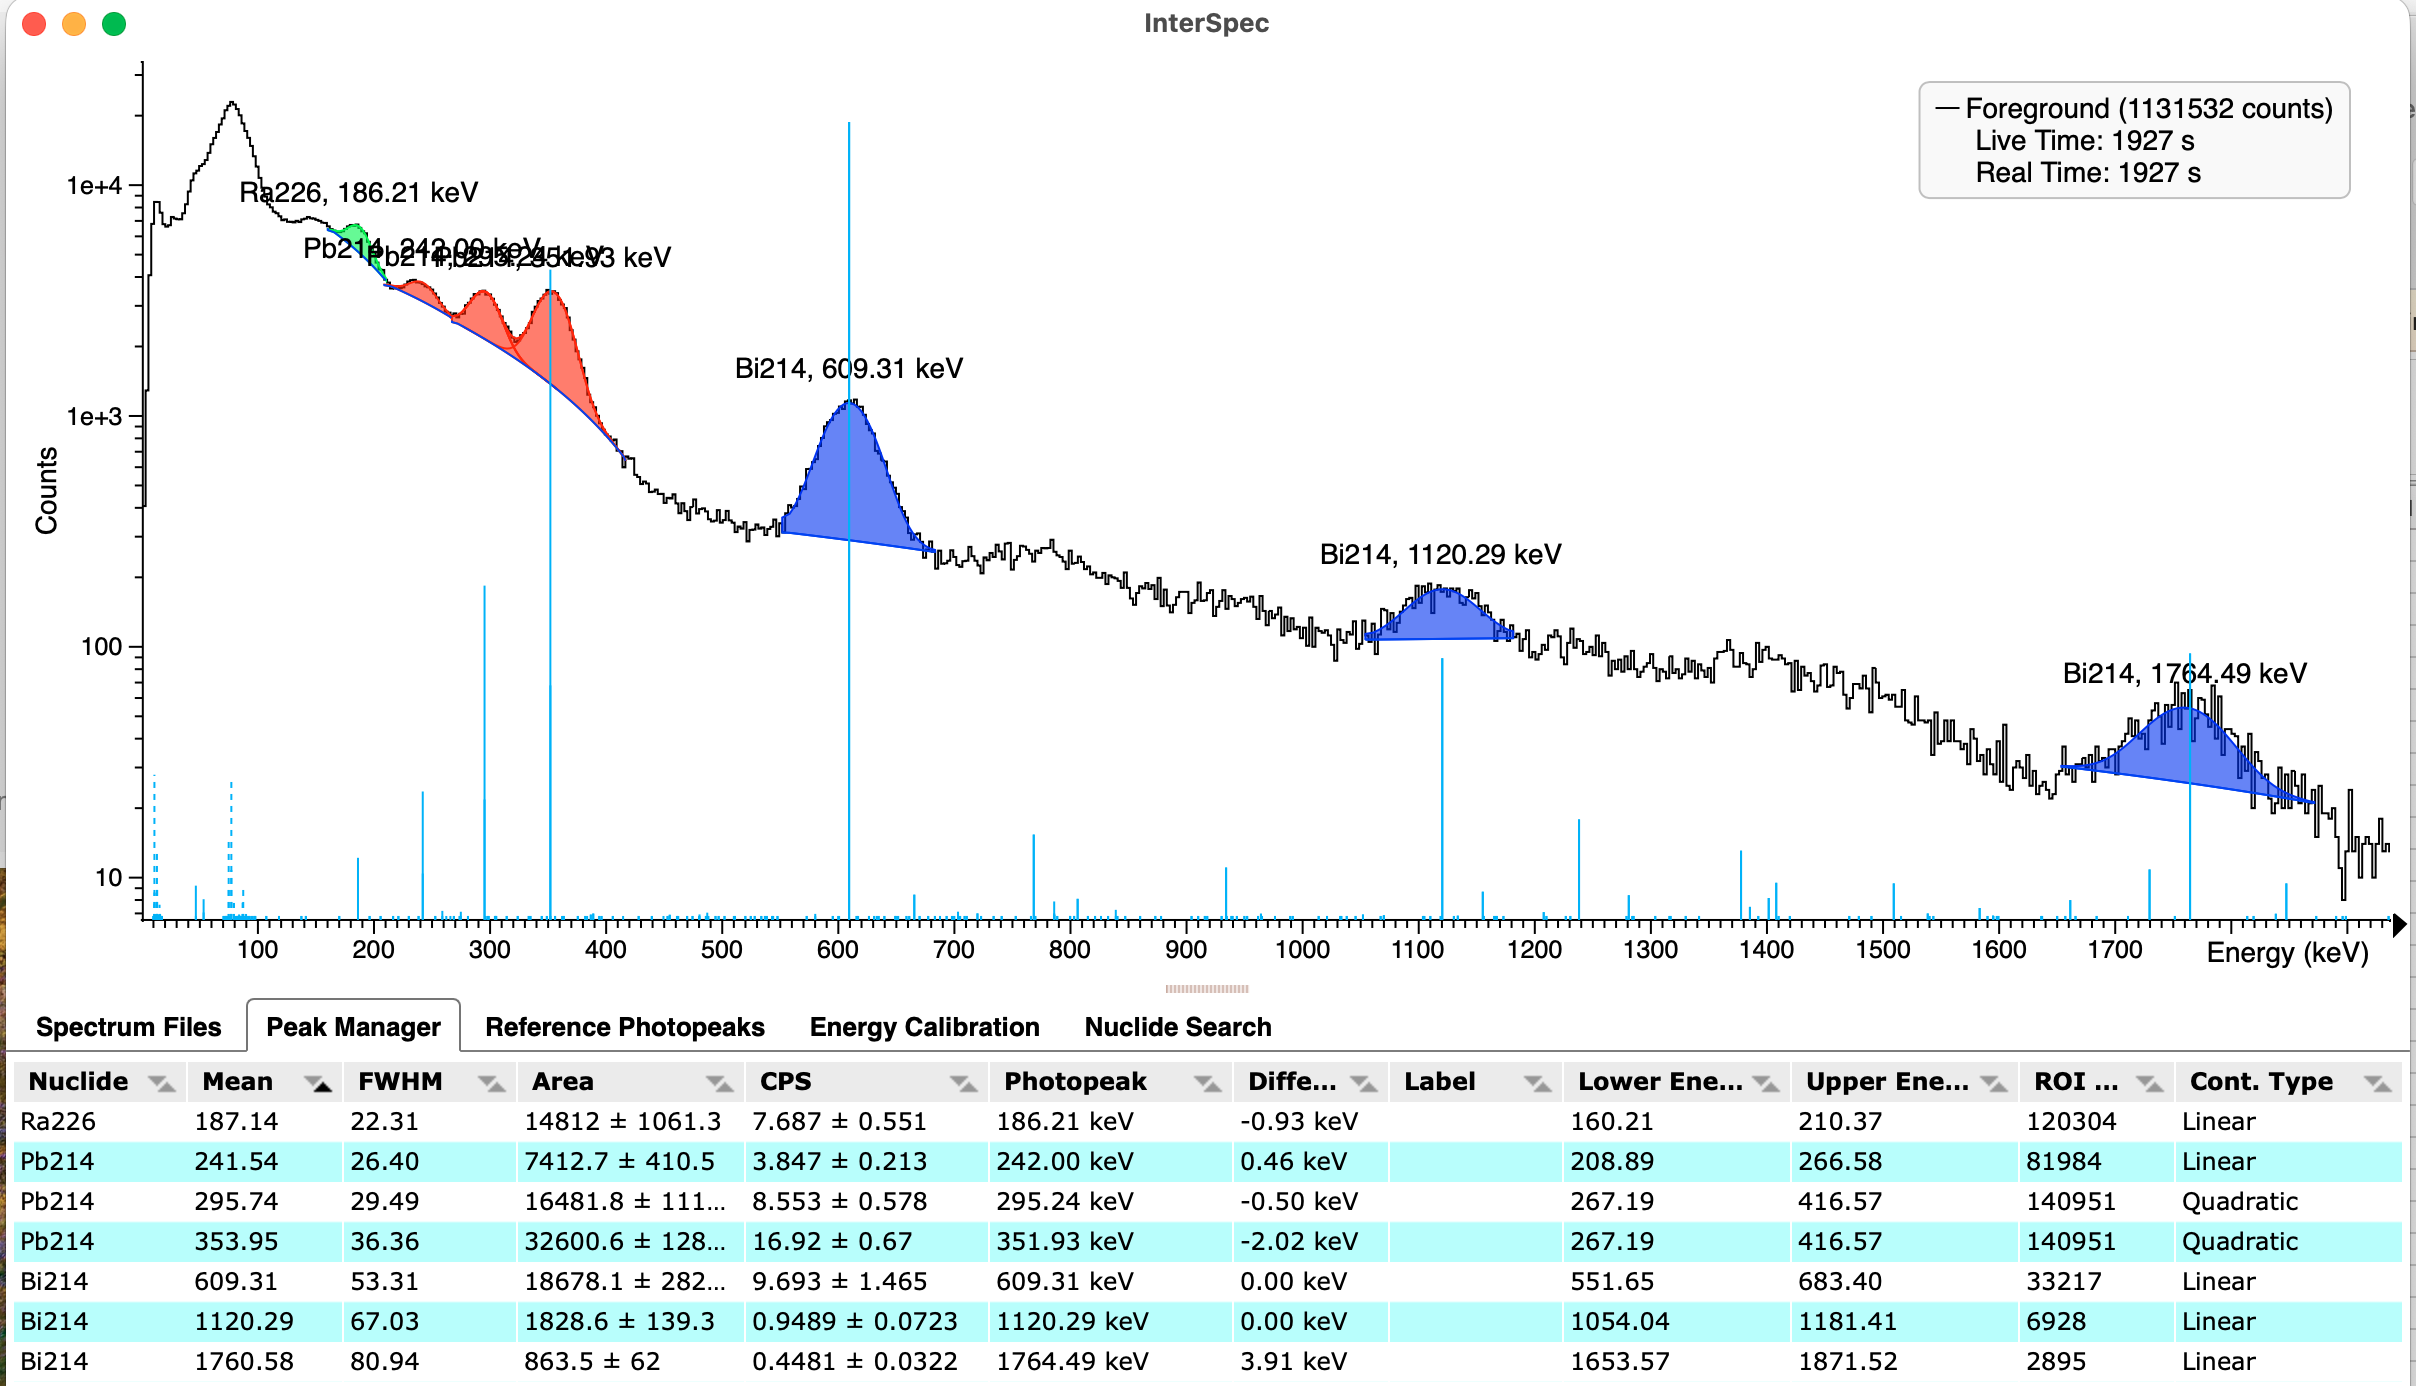
\includegraphics[width=0.95\textheight]{RadiumHigh.png}
    \caption{Typical high energy portion of the spectrum from measurement of the Radiacode in the radium jar. At a minimum you should report your measurements of the 7 $\gamma$ rays shown at the bottom of the figure, and described in Tab.~\ref{tab:radiumgam}.}
    \label{fig:RadiumHigh}
\end{sidewaysfigure}

In the heavy element radioactivity lab, you will measure a sample for depleted uranium, where the signal should be the $1001.0\,$keV $\gamma$ that follows the $\beta$ decay of $\elem{Pa}{234\text{m}}{91}{}{143}$.  This is the signature of the ``early chain" portion of the uranium chain.

You will also measure the spectrum of radium, from exposure in the radium jar at the front of the lab room.  The sample spectra you should observe, after uploading to Interspec, are shown in Figs.~\ref{fig:RadiumLow} and Figs.~\ref{fig:RadiumHigh}.  A table of the most prominent $\gamma$ rays in the radium chain are given in Tab.~\ref{tab:radiumgam}.

    \begin{table}[htbp]
      \centering
     \caption{Prominent $\gamma$ rays from the uranium decay chain, starting at radium, and their properties.  The branching ratio tells you what fraction of parent decays produce the $\gamma$ ray, and the cross section in our CsI detector for photoelectric absorption is $\sigma_A$.}
      \begin{tabular}{|c|c|c|c|} 
      \hline
        Parent & $\gamma\,E\,$(keV) & Branching Ratio (\%) & $\sigma_A$ in CsI (cm$^2$/g) \\ [0.5ex] 
        \hline\hline
$\elem{Ra}{226}{88}{}{138}$  &  186.8 & 3.28 & 0.306 \\
$\elem{Pb}{214}{82}{}{132}$  &  242.0  & 7.26 & 0.147 \\
$\elem{Pb}{214}{82}{}{132}$  &  295.2  & 18.4 & 0.0848 \\
$\elem{Pb}{214}{82}{}{132}$  &  351.9  & 35.6 & 0.0526 \\
$\elem{Bi}{214}{83}{}{131}$  &  609.3  & 45.4 & 0.0131 \\
$\elem{Bi}{214}{83}{}{131}$  &  1120  & 14.9 & 0.00348 \\
$\elem{Bi}{214}{83}{}{131}$  &  1764  & 15.3 & 0.00152 \\
       \hline
       \end{tabular}
\label{tab:radiumgam}
\end{table}

\FloatBarrier

\hbox{}
%\newpage

\subsubsection{The thorium chain}

The $\elem{Th}{232}{90}{}{142}$ chain is shown in Fig~\ref{fig:uchain}.  It starts in the upper middle, in the blue and yellow box with $\elem{Th}{232}{}{}{}$.

Thorium is about 3 to 4 times more abundant on Earth than uranium, and can also be used to make nuclear reactors and nuclear explosives.   It is less widely known than uranium, and has fewer decays, only 10, of which 6 are $\alpha$ decays, and 4 are $\beta$ decays, between the initial $\elem{Th}{232}{90}{}{142}$  and the final stable nuclide $\elem{Pb}{208}{82}{}{126}$.

One of the most interesting decays in the thorium chain is that of $\elem{Bi}{212}{83}{}{129}$, which decays about 2/3 of the time via $\beta$ decay to $\elem{Po}{212}{84}{}{128}$, and 1/3 of the time via $\alpha$ decay to $\elem{Tl}{208}{81}{}{127}$.

$\elem{Tl}{208}{81}{}{127}$ subsequently undergoes $\beta$ decay, usually to excited levels of $\elem{Pb}{208}{82}{}{126}$, and that nuclide decays by emission of $\gamma$ rays.  Among those $\gamma$ rays is one of the most energetic $\gamma$ rays from environmental radioactivity, with energy 2615~keV.

In Tab.~\ref{tab:thoriumgam}, you will find a list of the prominent $\gamma$ rays emitted in the thorium chain.  You should make a spectrum, with fits in Interspec, like Fig.~\ref{fig:thorium}, and report your results.

The fun property of the 2615~keV $\gamma$ ray is that it has an energy so large that it can actually produce antimatter.  That $\gamma$ ray, in the strong electric field of either the cesium or iodine nucleus of the Radiacode, can produce a positron ($e^+$, rest energy 511~keV) and an electron (rest energy also 511~keV), for a total of $1022$~keV needed.  That leaves 2615-1022=1593~keV which goes into kinetic energy of the electron and positron, which is extremely close the the 1588~keV gamma ray in the sixth row of Tab.~\ref{tab:thoriumgam}.

Sometimes the positron finds an electron in the CsI, they annihilate, and the $\gamma$ rays produced escape the CsI crystal, losing $1022$~keV.  This is called the ``double escape peak"... can you find evidence for that peak in your thorium spectrum?   To do so, look carefully at the counts-per-second of what is called the 1588~keV peak.   That is: try to figure out numerically if the counts-per-second you measure is much larger than the expectation based on Tab.~\ref{tab:thoriumgam}.

A quick test of the importance of $e^+e^-$ production by the 2615~keV $\gamma$-ray: look at the cross section for pair production in the nuclear field in XCOM.  If you do that, you find that the cross section is 0.005843~cm$^2$/g, which is 7.3 times larger than the photoelectric absorption cross section.  So $e^+e^-$ pair production is a substantial process.

There is also a feature in the thorium spectrum from escape of one of the $\gamma$ rays from annihilation of the $e^+$, near 2615-511=2104~keV.  This feature is just below the Compton edge of the 2615~keV $\gamma$ ray, which is at 2382~keV, and is called the ``single escape peak".

A challenge-type problem: describe the evidence for positrons in your thorium spectrum (like Fig.~\ref{fig:thorium}), with numbers to back up your case.



\begin{sidewaysfigure}
    \centering
    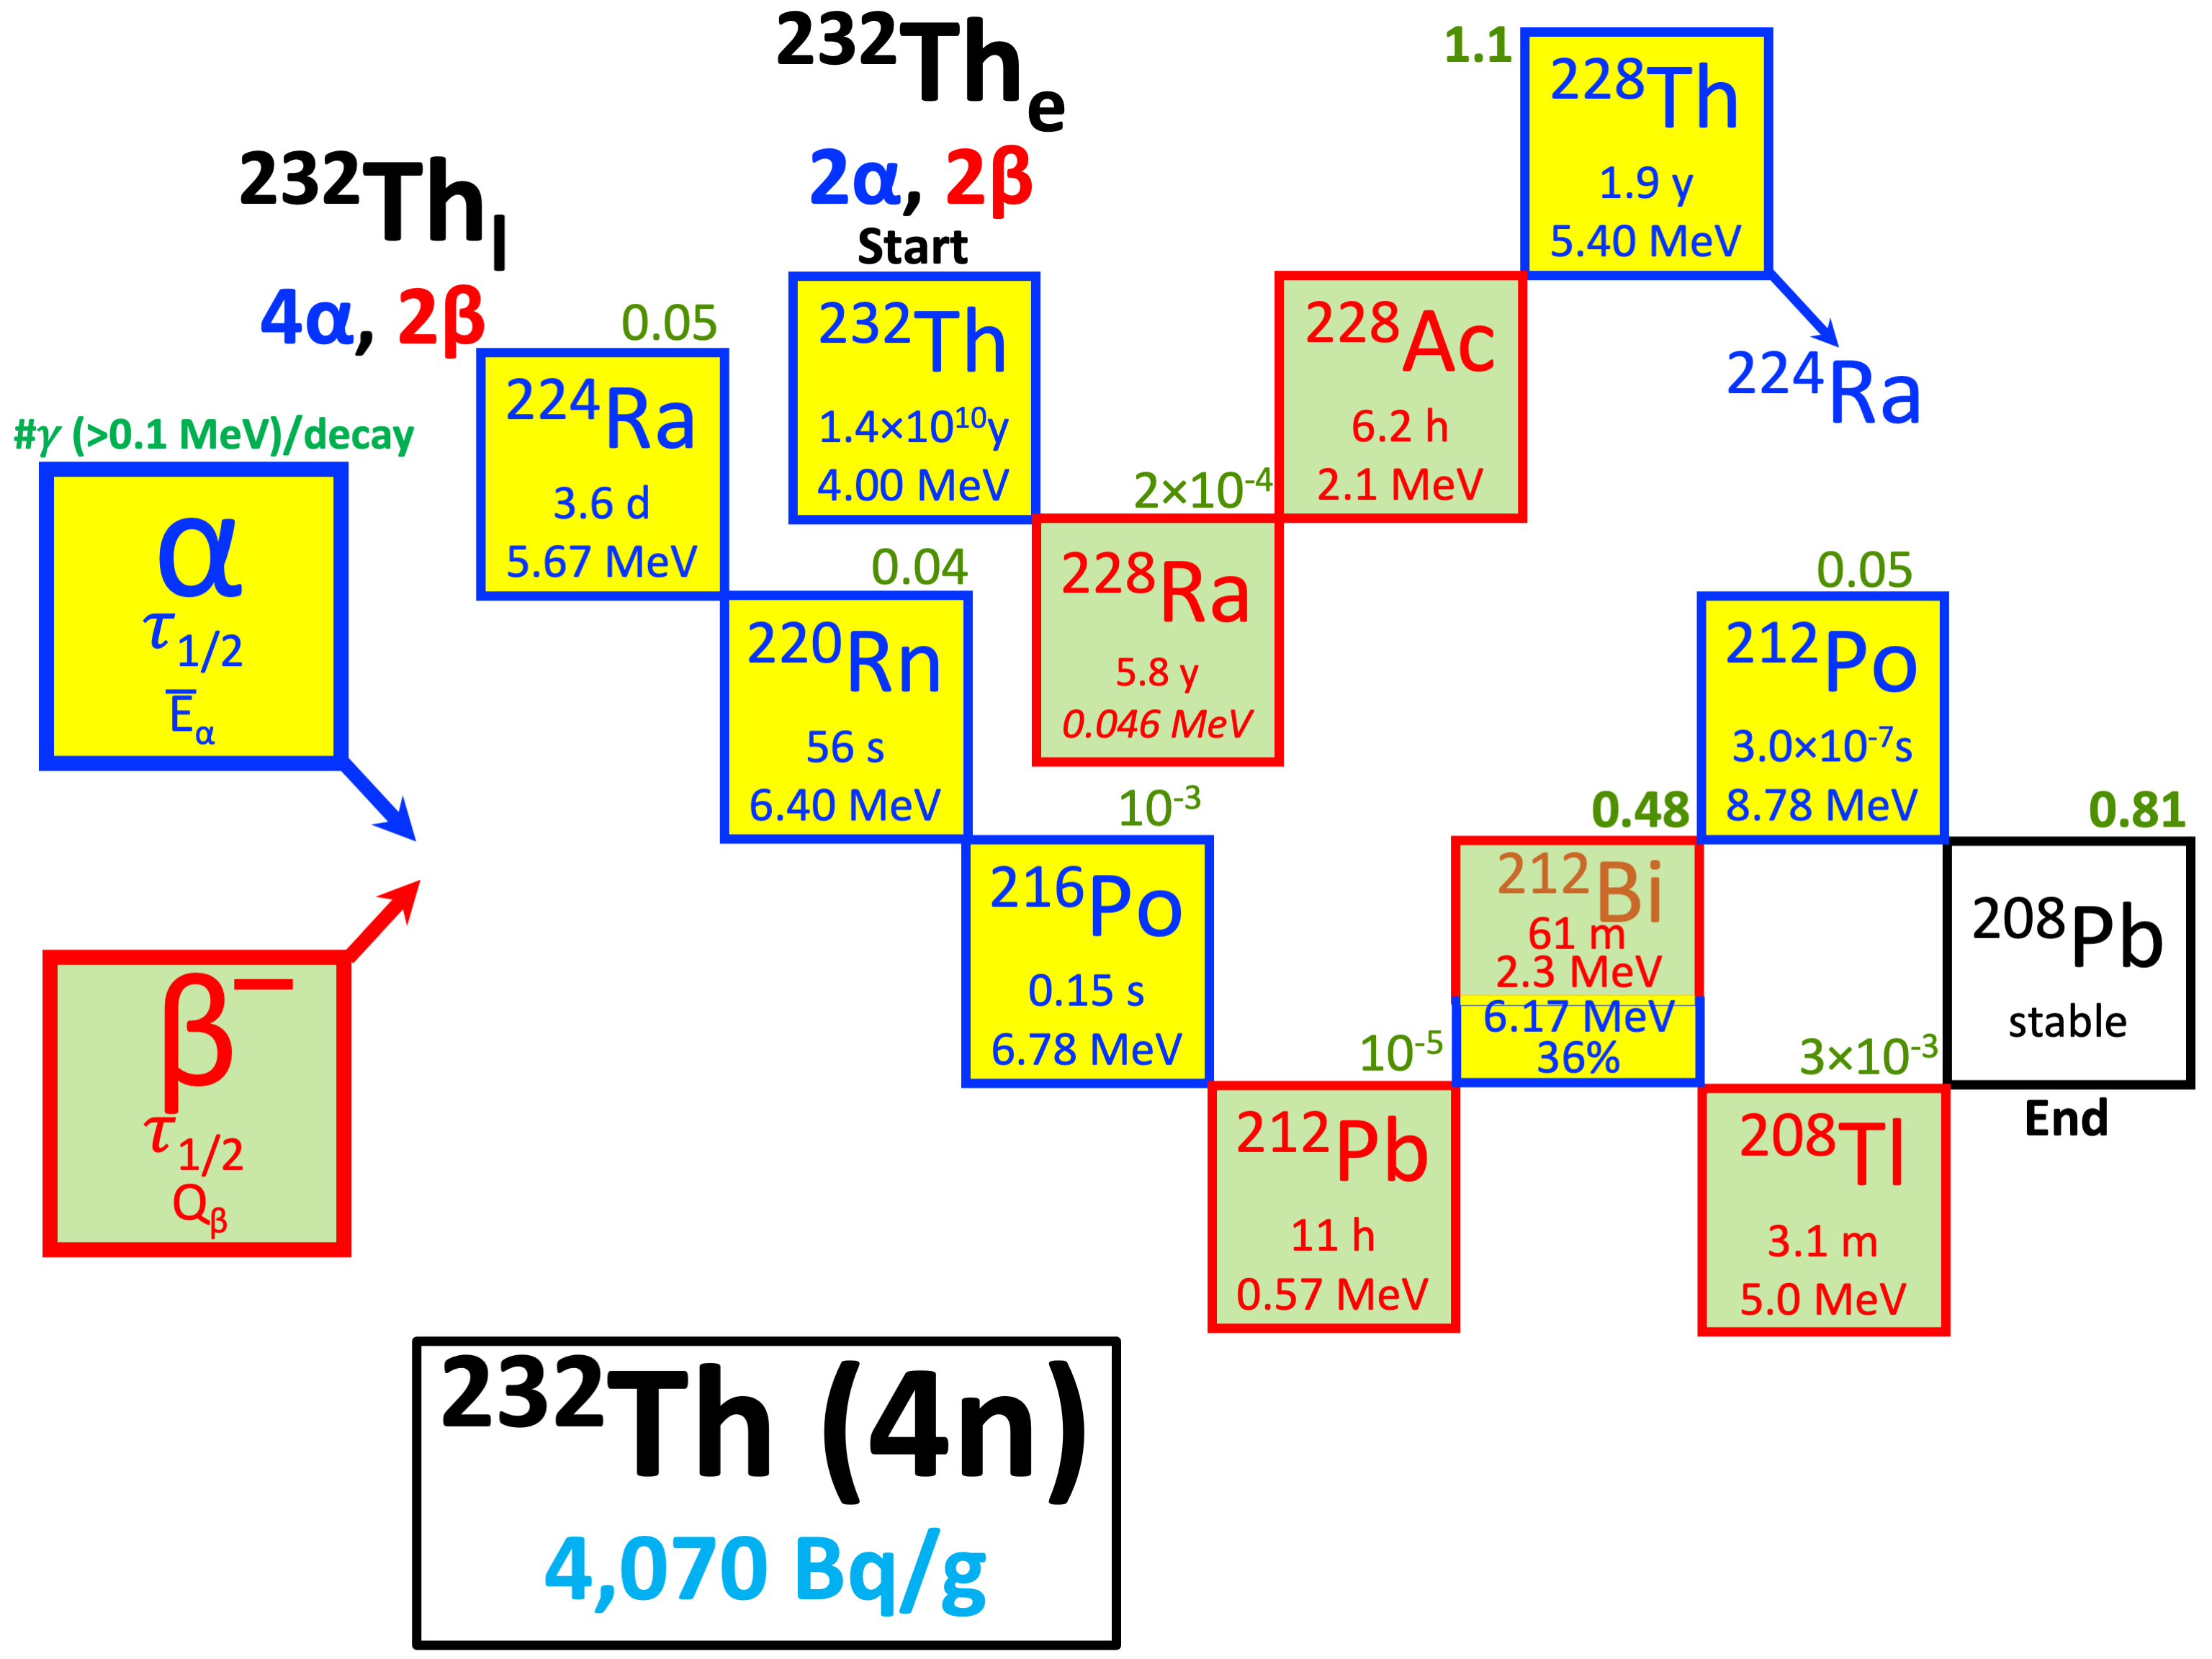
\includegraphics[width=0.95\textheight]{Th232Chain.png}
    \caption{The $\elem{Th}{232}{90}{}{142}$ decay chain.  The green numbers above each box show how many $\gamma$ rays are emitted per decay.  The way to read the chart is: the $\beta$ decay of $\elem{Ac}{228}{89}{}{139}$ goes to an excited state of $\elem{Th}{228}{90}{}{138}$, which on average emit 1.1 $\gamma$ rays per $\beta$ decay.  More than one $\gamma$ per $\beta$ decay can be emitted because there is often a cascade of multiple $\gamma$'s as the excited $\elem{Th}{228}{90}{}{138}$ decays.}
    \label{fig:thchain}
\end{sidewaysfigure}

\begin{table}[htbp]
      \centering
     \caption{Prominent $\gamma$ rays from the thorium decay chain and their properties.  The branching ratio tells you what fraction of parent decays produce the $\gamma$ ray, and the cross section in our CsI detector for photoelectric absorption is $\sigma_A$.}
      \begin{tabular}{|c|c|c|c|} 
      \hline
        Parent & $\gamma\,E\,$(keV) & Branching Ratio (\%) & $\sigma_A$ in CsI (cm$^2$/g) \\ [0.5ex] 
        \hline\hline
$\elem{Pb}{212}{82}{}{130}$  &  238.6 & 43.6 & 0.153 \\
$\elem{Ac}{228}{89}{}{139}$  &  338.3  & 11.3 & 0.0585 \\
$\elem{Tl}{208}{81}{}{127}$  &  510.8  & 8.12 & 0.0201 \\
$\elem{Ac}{228}{89}{}{139}$  &  911.2 & 25.8 & 0.00534 \\
$\elem{Ac}{228}{89}{}{139}$  &  969.0  & 15.8 & 0.00469 \\
$\elem{Ac}{228}{89}{}{139}$  &  1588  & 3.22 & 0.00183 \\
$\elem{Tl}{208}{81}{}{127}$  &  2615 & 35.9 & 0.000803 \\
       \hline
       \end{tabular}
\label{tab:thoriumgam}
\end{table}

\begin{sidewaysfigure}
    \centering
    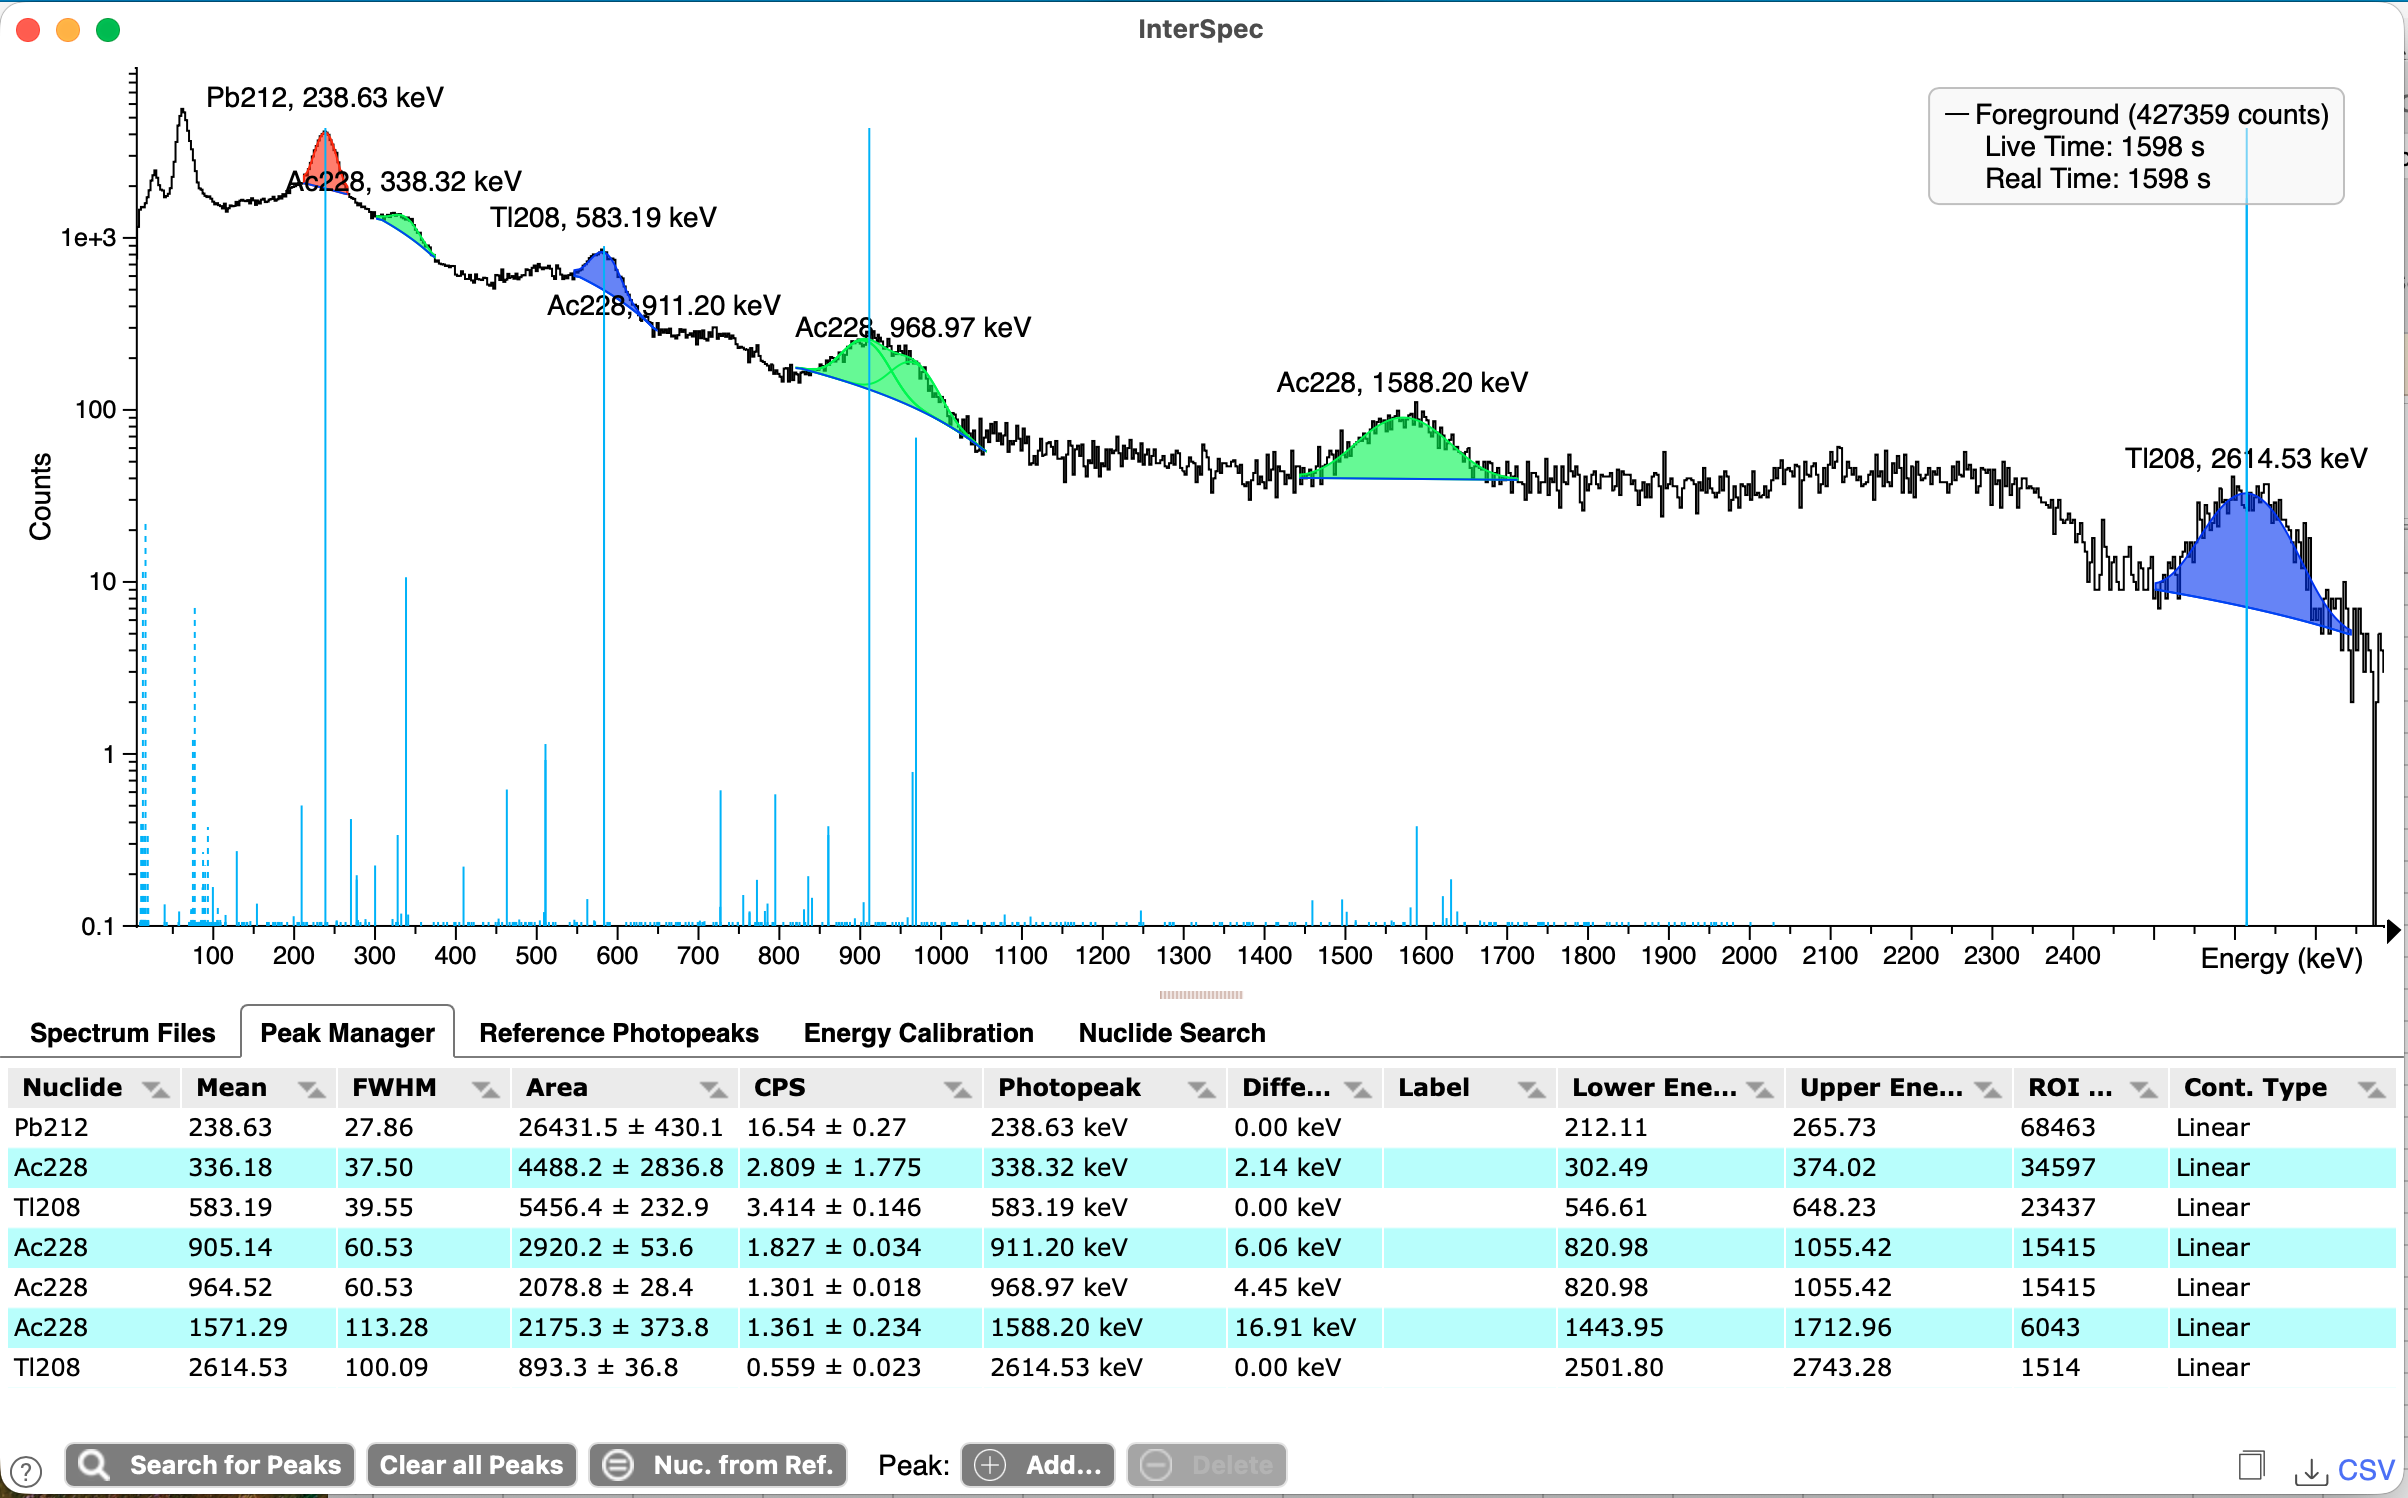
\includegraphics[width=0.95\textheight]{Thorium.png}
    \caption{Typical  spectrum from measurement of the Radiacode exposed to thorium. At a minimum you should report your measurements of the 7 $\gamma$ rays shown at the bottom of the figure, and described in Tab.~\ref{tab:thoriumgam}.}
    \label{fig:thorium}
\end{sidewaysfigure}



\end{document}